\section*{Preamble to Chapter~\ref{chap:manuscript}}

The following chapter reproduces the manuscript entitled
``\textit{Hybrid GNN–Tree Models for Optical Property Prediction: Decoupling Representation and Regression in Low-Data Regimes}'' 
by Michael Montemurri, Shambhavi Tannir, and Eric Kolaczyk. 
This work is intended for submission to the \textit{Journal of Chemical Information and Modeling}.

The research presented in this chapter constitutes the primary original contribution of this thesis. The candidate was responsible for the conceptual development, implementation, experimental design, empirical analysis, and preparation of the manuscript. Collaborators provided guidance on interpretation and scientific framing.

The manuscript is reproduced here in full, with minor formatting adjustments for consistency with thesis style (e.g., figure numbering and section references). 

This chapter builds on the theoretical and methodological foundations established in Chapters 2 and 3 and presents the empirical evaluation and comparative analysis of the classical, D-MPNN, and hybrid modelling frameworks.

\section{Introduction}
Machine learning models are now widely used for molecular property prediction (MPP), offering a data-driven alternative to quantum chemical simulation and experimental screening in areas such as drug discovery, materials science, and photophysical materials design~\cite{butler2018machine, schneider2020rethinking, jha2018elemnet}. Deep learning approaches that learn structure–property relationships directly from molecular graphs have achieved state-of-the-art performance across a wide array of MPP benchmarks~\cite{ying2021transformers, hu2020open, gasteiger2020directional}.

Despite these successes, the practical utility of deep models is frequently constrained by data availability. Experimental research groups often operate in a ``low-data'' regime, generating task-specific datasets ranging from tens to a few thousand molecules. A variety of deep learning architectures have been applied to MPP tasks, including sequence-based models operating on string-based representations and graph-based models operating directly on molecular structure. Among these, graph neural networks (GNNs) have emerged as a dominant paradigm because they incorporate molecular topology as an explicit inductive bias. However, in low-data settings, end-to-end GNNs often exhibit unstable training dynamics, high sensitivity to random initialization, and poor generalization under distribution shift~\cite{chuang2020debiased, grinsztajn2022tree}. This raises critical questions about the efficacy of GNN-based deep learning relative to simpler baselines when labeled data is scarce.

These challenges are particularly prevalent in the prediction of optical properties, such as absorption and emission wavelengths, which are vital for organic electronics, photonic materials, and fluorescent probes~\cite{facchetti2011pi}. Unlike ground-state properties (e.g., solubility or toxicity), optical responses are governed by excited-state electronic structure, which depends sensitively on $\pi$-conjugation length, solvent environment, and conformational flexibility~\cite{lakowicz2006principles, martin2020electronic, reichardt2011solvents}. Small structural modifications can yield large, non-intuitive spectral shifts, creating ``activity cliffs'' that are difficult for smooth, continuous models to capture without dense sampling~\cite{van2022exposing}.

While quantum chemical methods such as Time-Dependent Density Functional Theory (TD-DFT) provide physically grounded estimates of excited-state properties, they scale poorly with both molecule and dataset size, requiring substantial computational resources~\cite{dreuw2005single, casida2009time}. Tannir \textit{et al.} demonstrate that descriptor-based gradient-boosted ensembles can achieve strong performance on curated optical datasets when augmented with handcrafted TD-DFT–derived features~\cite{tannir2024predicting}. However, such approaches depend on computing quantum-chemical descriptors for each molecule at inference time, limiting their applicability in large-scale screening. To retain the informational benefits of quantum calculations without incurring inference-time costs, recent work by Greenman \textit{et al.} has explored multi-fidelity strategies that train machine learning surrogates jointly on experimental and computational datasets to avoid the need for DFT calculations at inference~\cite{greenman2022multi, ramakrishnan2015big}.

Conversely, in purely experimental low-data regimes, classical models based on fixed molecular descriptors (e.g., Morgan fingerprints) often outperform deep learning approaches due to their strong inductive biases and statistical efficiency~\cite{rogers2010extended, wu2018moleculenet, xia2023understanding}. However, these approaches may fail to capture the higher-order structural effects and long-range dependencies relevant to optical response.

Transfer learning has been proposed as a remedy for the lack of labeled data, but its effectiveness for molecular regression tasks is highly regime-dependent. Recent studies indicate that without strict chemical alignment between pretraining and downstream tasks, transfer learning can yield negligible or even negative transfer, particularly in regression tasks involving distinct physical mechanisms~\cite{hu2019strategies, sun2022does, buterez2024transfer}.

To balance the expressive power of GNNs with the statistical stability of classical regression, researchers are increasingly adopting hybrid modelling strategies. For instance, Deng \textit{et al.} introduced XGraphBoost, a framework that utilizes GNN-learned representations as input features for Gradient-Boosted Decision Trees (GBDTs). Their comprehensive benchmark evaluation identified the combination of eXtreme Gradient Boosting (XGB) with a Directed Message Passing Neural Network (D-MPNN) as the top-performing hybrid strategy~\cite{deng2021xgraphboost,chen2016xgboost,yang2019analyzing}. While this work establishes the promise of hybrid architectures, it does not address the regimes most relevant to experimental photophysics, where datasets are small, domain-specific, and often subject to distribution shift. Moreover, prior hybrid studies have largely focused on aggregate benchmark performance, without examining how predictive accuracy, variance, and learned representations evolve as a function of dataset size.

Hybrid models explicitly decouple representation learning from downstream regression, making the structure of the learned embedding space a central object of study rather than a hidden intermediate. In low-data regimes, where models are prone to memorizing noise rather than learning generalizable features, it is imperative to ensure that learned representations capture chemically meaningful structure rather than overfitting to the limited training data. 

In this work, we systematically evaluate a suite of classical, D-MPNN, and hybrid modelling strategies for optical property prediction across multiple datasets, data regimes, and train–test splits. We compare end-to-end D-MPNNs with hybrid models that use D-MPNN embeddings to train lightweight tree-based heads. We demonstrate that hybrid models broadly outperform end-to-end D-MPNNs on peak absorption wavelength prediction in small-data regimes. Through controlled transfer learning experiments, we show that the benefits of pretraining are strongly regime- and coverage-dependent, yielding substantial gains on chemically aligned downstream datasets but limited or negative returns under significant distribution shift. Furthermore, using a nested experimental design, we decompose predictive variability into contributions arising from representation learning and downstream prediction; we find that while predictive instability is dominated by representation learning across regimes, the downstream head contributes a substantial fraction in data-limited settings. Finally, we analyze the structure of learned molecular embeddings and demonstrate that these representations retain chemically meaningful organization aligned with known determinants of optical response, providing practical guidance for modelling optical properties in small and specialized chemical datasets.


\section{Background and Methods}
\label{sec:methods}
This section presents the modelling framework and analytical procedures used throughout this work, focusing on methodological components that are agnostic to dataset and experimental setting. Dataset-specific design choices, training regimes, and evaluation protocols are treated separately.

\subsection{Graph Neural Network Encoder}

Molecules are represented as graphs $G = (V, E)$, where nodes $v \in V$ correspond to atoms and edges $(v,u) \in E$ correspond to chemical bonds. Following Yang \textit{et al.}~\cite{yang2019analyzing}, we initialize our feature vectors with the standard RDKit atom- and bond-level features listed explicitly in Tables~\ref{tab:atom-features} and~\ref{tab:bond-features}. 

We employ a D-MPNN as the molecular graph encoder using the Chemprop open-source package (version 1.6.1)~\cite{yang2019analyzing}. In contrast to atom-centered message passing, the D-MPNN propagates messages along directed bonds to prevent message backtracking. For a directed bond from atom $v$ to atom $u$, the initial message $\mathbf{h}_{vu}^{(0)}$ is computed using the features of the source atom $v$ and the bond $(v,u)$:
\begin{equation}
\mathbf{h}_{vu}^{(0)} = \sigma(\mathbf{W}_i [\mathbf{x}_v \,\|\, \mathbf{b}_{vu}]),
\end{equation}
where $\mathbf{x}_v$ and $\mathbf{b}_{vu}$ denote atom and bond feature vectors, respectively, $\|$ denotes concatenation, $\sigma$ denotes the ReLU activation function, and $\mathbf{W}_i$ is a learned initial linear transformation mapping features into a shared $d$-dimensional hidden space, where $d$ is a chosen hyperparameter.


In each message-passing step $t \in \{1, \dots, T\}$, the hidden state $\mathbf{h}_{vu}^{(t)}$ is updated by aggregating messages from all incoming directed bonds $(k,v)$ except for the reverse bond $(u,v)$:
\begin{equation}
\mathbf{h}_{vu}^{(t+1)} = \sigma \!\left(
\mathbf{h}_{vu}^{(0)} + \mathbf{W}_h
\sum_{k \in \mathcal{N}(v) \setminus \{u\}} \mathbf{h}_{kv}^{(t)}
\right),
\end{equation}
where $\mathcal{N}(v)$ denotes the neighbours of atom $v$, and $\mathbf{W}_h \in \mathbb{R}^{d \times d}$ is a learned weight matrix shared across all steps.


After $T$ iterations, the bond-level messages are aggregated to form atom-level representations $\mathbf{h}_u$. The original atom features $\mathbf{x}_u$ are concatenated with the summed incoming bond messages and passed through a final linear layer:
\begin{equation}
\mathbf{h}_u = \sigma \!\left( \mathbf{W}_a \left[ \mathbf{x}_u \,\|\, \sum_{v \in \mathcal{N}(u)} \mathbf{h}_{vu}^{(T)} \right] \right).
\end{equation}
The global molecular embedding $\mathbf{z}_{\mathrm{mol}} \in \mathbb{R}^d$ is then computed via global sum pooling, yielding a permutation-invariant representation of the molecular graph:
\begin{equation}
\mathbf{z}_\mathrm{mol} = \sum_{u \in V} \mathbf{h}_u.
\end{equation}

Let $\mathbf z_{\mathrm{sol}}$ denote the fixed solvent representation. The full representation used for downstream prediction is
\begin{equation}
\mathbf z = [\mathbf z_{\mathrm{mol}} \,\|\, \mathbf z_{\mathrm{sol}}].
\end{equation}

Throughout this work, we refer to the mapping from this combined representation to the scalar property prediction as the head. In the end-to-end setting, this head is a neural feedforward network (FFN), whereas in the hybrid setting it is replaced by a separate gradient-boosted tree model.


\subsection{End-to-End and Hybrid Modelling Paradigms}

\begin{figure}[t!]
    \centering
    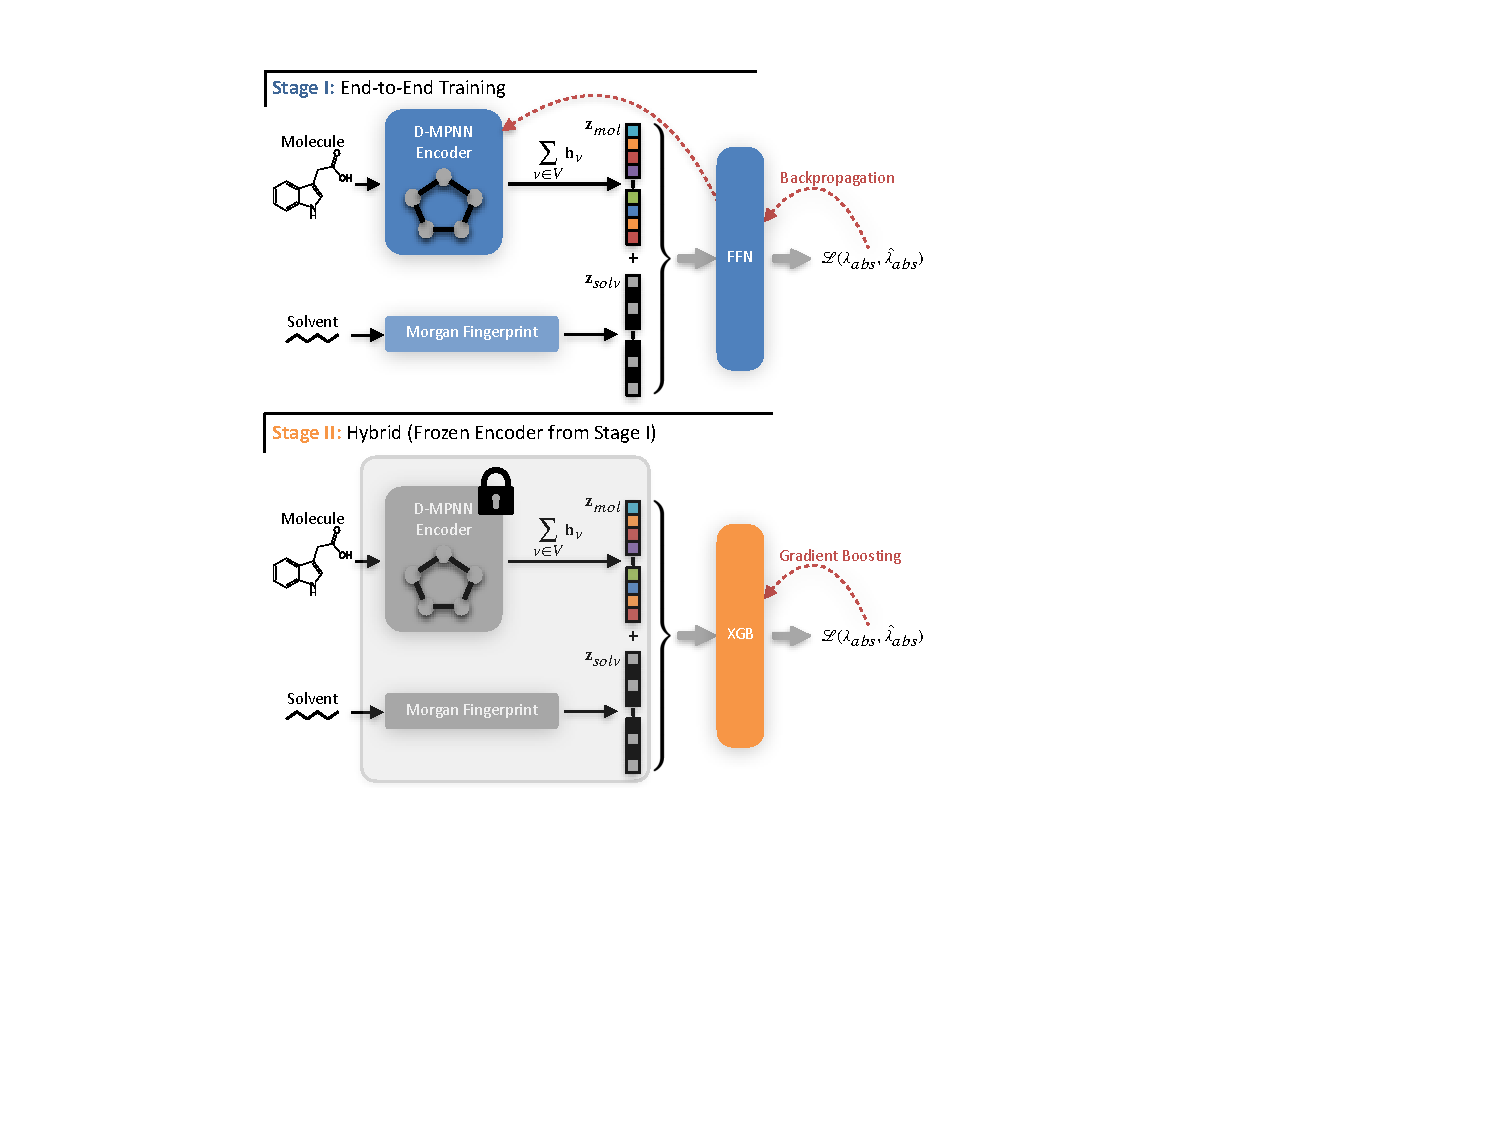
\includegraphics[width=0.8\linewidth]{figures/hybrid_end2end_architecture_schematic.pdf}
    \caption{\textbf{Two-stage hybrid modelling framework.} 
    \textbf{Stage I (Top):} A D-MPNN encoder maps the molecular graph to per-atom hidden states, which are aggregated via sum pooling to form a molecular representation ($\mathbf{z}_{\mathrm{mol}}$). This representation is concatenated with fixed solvent Morgan fingerprints ($\mathbf{z}_{\mathrm{sol}}$) and used to train a feedforward neural network (FFN) in an end-to-end manner, with gradients of the training loss propagated through both the FFN and encoder. 
    \textbf{Stage II (Bottom):} The pretrained D-MPNN encoder from Stage~I is frozen and reused to generate molecular representations ($\mathbf z_{\mathrm{mol}}$), which are again concatenated with solvent fingerprints ($\mathbf z_{\mathrm{sol}}$) and used as fixed features for an XGBoost head.}
    \label{fig:hybrid_schematic}
\end{figure}

We consider two modelling paradigms built upon the same D-MPNN encoder $\phi_{\theta}$ with parameters $\theta$, depicted in Figure~\ref{fig:hybrid_schematic}.

In the end-to-end paradigm, the molecular embedding $\mathbf z_{\mathrm{mol}} = \phi_\theta(G)
$ and solvent embedding $\mathbf z_{\mathrm{sol}}$ are concatenated and passed to a feedforward neural network (FFN) head $g_{\psi}(\cdot)$, and all parameters $\{\theta, \psi\}$ are optimized jointly:
\begin{equation}
\hat{y}_{\text{E2E}} = g_\psi(\mathbf z)
= g_{\psi}(\phi_{\theta}(G), \mathbf z_{\mathrm{sol}}).
\end{equation}

Given training data $\{(G_i,\mathbf z_{\mathrm{sol},i},y_i)\}_{i=1}^N$, parameters are learned by minimizing the empirical risk
\begin{equation}
\mathcal{L}(\theta,\psi)
=
\frac{1}{N} \sum_{i=1}^{N}
\ell\!\left(
y_i,
g_{\psi}(\phi_{\theta}(G_i), \mathbf z_{\mathrm{sol},i})
\right),
\end{equation}
where $\ell(\cdot,\cdot)$ denotes the task-specific loss function (mean squared error for regression in our experiments). Gradients of $\mathcal{L}$ are computed with respect to both encoder parameters $\theta$ and head parameters $\psi$.

This approach allows the learned representation to adapt directly to the prediction task but may introduce instability in low-data regimes due to the high-dimensional parameter space.

In the hybrid paradigm, we train the full encoder--head model, $g_{\psi}(\phi_{\theta}(G),\mathbf z_{\mathrm{sol}})$, end-to-end on the downstream task. After learning the parameters, we discard the FFN head $g_{\psi}(\cdot)$ and freeze the encoder $\phi_{\theta^*}(G)$, where $\theta^*$ indicates that the parameters are frozen. Predictions are then generated by a separate regression head $h_{\omega}$:
\begin{equation}
\hat{y}_{\text{hybrid}} = h_{\omega}(\phi_{\theta^*}(G),\mathbf z_{\mathrm{sol}}),
\end{equation}
where only the head parameters $\omega$ are optimized in the second-stage regression step. Decoupling representation learning from regression enables the use of models with different inductive biases, such as gradient-boosted trees, while ensuring that all comparisons are performed on the same frozen molecular embeddings augmented with identical solvent covariates.

\subsection{Downstream Regression via Gradient Boosting}
In our hybrid framework, we utilize XGBoost~\cite{chen2016xgboost} to serve as a regularized non-linear head for the frozen D-MPNN embeddings. Unlike the multi-layer perceptrons typically used in end-to-end GNNs, XGBoost constructs an additive ensemble of decision trees that incorporates explicit regularization on tree complexity (e.g., minimum split loss ($\gamma$) and leaf weights ($\lambda$)). This structural regularization is particularly advantageous in the data-limited regimes characteristic of experimental photophysics, where overparameterized neural heads are prone to overfitting.


\subsection{Baseline Models}

We evaluated several baseline approaches common to molecular property prediction. All baseline models were trained and evaluated using the same canonical data splits, fixed training subsamples, and evaluation protocols as the D-MPNN-based models.


\paragraph{Fingerprint-based baselines.}
As a classical cheminformatics baseline, molecules were represented using fixed-length Morgan fingerprints (radius 2, 2048 bits) computed with RDKit. Solvents were represented using separate Morgan fingerprints (radius 2, 1024 bits) which were concatenated with the molecular fingerprints. This concatenation strategy mirrors the solvent integration used in the D-MPNN and hybrid architectures, ensuring that all models have access to equivalent environmental context. To capture global physicochemical properties often missed by substructure fingerprints, we additionally explored augmenting these vectors with nine scalar descriptors: molecular weight (MolWt), octanol--water partition coefficient (MolLogP), topological polar surface area (TPSA), hydrogen bond acceptor and donor counts (HBA/HBD), aromatic and aliphatic ring counts, rotatable bond count, and the fraction of $sp^3$-hybridized carbon atoms ($f_{sp^3}$). These tabular representations were used to train a suite of regression models: ridge and polynomial regressions, Random Forests, and XGBoost models.

\paragraph{Physics-informed baselines.}
We evaluated the predictive utility of low-fidelity quantum-chemical (QC) descriptors derived from density functional theory calculations reported by Greenman \textit{et al.}~\cite{greenman2022multi}. In that work, molecular geometries were generated from SMILES strings and optimized using a multistage pipeline including semi-empirical tight-binding (GFN2-xTB), followed by DFT geometry optimization at the BP86-D3/def2-SVP level. TD-DFT calculations were then performed using the Tamm--Dancoff approximation at the $\omega$B97X-D3/def2-SVPD level of theory to estimate vertical excitation energies. For a subset of dye--solvent pairs, additional solvent-corrected TD-DFT calculations were carried out using the IEFPCM continuum solvation model. 

While these descriptors provide valuable physical signal, they require nontrivial QC calculations and are therefore substantially more expensive than purely data-driven representations. Accordingly, these baselines are included to contextualize the performance of learned representations relative to low-fidelity physics, rather than as a practical alternative in large-scale or low-latency settings.

Motivated by Tannir \textit{et al.}~\cite{tannir2024predicting}, we utilize the resulting HOMO--LUMO gap estimates as physics-informed descriptors. For molecules where this information was not available ($\leq 2\%$), we employ median imputation. These QC features were combined with fingerprint-based representations and used as inputs to the same downstream regression models, enabling direct comparison between learned representations, purely empirical features, and hybrid physics-informed baselines.

Finally, we evaluated a minimal parametric model motivated by Frontier Molecular Orbital (FMO) theory. Approximating the dominant optical transition energy by the energy gap between the highest occupied molecular orbital (HOMO) and the lowest unoccupied molecular orbital (LUMO), and invoking the Planck--Einstein relation ($E = hc/\lambda$), we fit an inverse-gap regression of the form:
\begin{equation}
\lambda_{\max} \approx \beta_0 + \beta_1 (\Delta \epsilon_{\text{H--L}})^{-1},
\end{equation}
to establish a predictive baseline rooted in first-principles physics. While this approximation neglects vibronic structure, excited-state relaxation, and explicit solvent reorganization, it provides a useful low-capacity benchmark against which more expressive learned representations can be evaluated.


For standard fingerprint- and descriptor-based baselines, we performed hyperparameter optimization using Optuna, utilizing the validation set for model selection. In contrast, the DFT-informed baselines were trained using default hyperparameters; consequently, we combined the training and validation sets for these models to maximize data utilization during fitting. Regardless of the training protocol, the test set was strictly reserved for final evaluation to ensure fair comparison across all architectures.

\subsection{Variance Decomposition Framework}
\label{subsec:var-decomp}

\begin{figure}[ht]
    \centering
    \begin{tikzpicture}[
    scale=0.7, transform shape,
    % Standardizes node styles
    encoder/.style={circle, draw=encodercolor, fill=encodercolor!10, thick, inner sep=2pt, minimum size=0.8cm},
    hpo/.style={rectangle, draw=hpocolor, fill=hpocolor!10, thick, rounded corners=2pt, inner sep=4pt},
    residual/.style={text=seedcolor, font=\small}, % Changed from \scriptsize\ttfamily
    % Tree geometry
    level 1/.style={sibling distance=2.4cm, level distance=1.2cm},
    level 2/.style={sibling distance=1.2cm, level distance=2.0cm},
    level 3/.style={sibling distance=0.7cm, level distance=1.4cm},
    edge from parent/.style={draw, -latex', gray!60, thick}
]

% Root node
\node[draw, rectangle, rounded corners=3pt, thick, inner sep=6pt, fill=gray!5] (root) {Training Data}
child {node[encoder] {$A_1$}
    % HPO Config 1 (j=1, i=1)
    child {node[hpo] {$B_{1(1)}$}
        child {node[residual] {$\varepsilon_{1(11)}$}} % Correct: k=1, j=1, i=1
        child {node[residual] {$\dots$}}
        child {node[residual] {$\varepsilon_{5(11)}$}} % Correct: k=5, j=1, i=1
    }
    child {node[gray!50, font=\Large] {$\dots$}}
    % HPO Config 5 (j=5, i=1)
    child {node[hpo] {$B_{5(1)}$}
        child {node[residual] {$\varepsilon_{1(51)}$}} % Correct: k=1, j=5, i=1
        child {node[residual] {$\dots$}}
        child {node[residual] {$\varepsilon_{5(51)}$}} % Correct: k=5, j=5, i=1
    }
}
    % Represent the gap to the 5th encoder
    child {node[gray!50, font=\Large, yshift=-0.5cm] {$\dots$} child[missing]}
% Encoder 5 branch (i=5)
child {node[encoder] {$A_5$}
    % HPO Config 1 (j=1, i=5)
    child {node[hpo] {$B_{1(5)}$}
        child {node[residual] {$\varepsilon_{1(15)}$}} % Correct: k=1, j=1, i=5
        child {node[residual] {$\dots$}}
        child {node[residual] {$\varepsilon_{5(15)}$}} % Correct: k=5, j=1, i=5
    }
    child {node[gray!50, font=\Large] {$\dots$}}
    % HPO Config 5 (j=5, i=5)
    child {node[hpo] {$B_{5(5)}$}
        child {node[residual] {$\varepsilon_{1(55)}$}} % Correct: k=1, j=5, i=5
        child {node[residual] {$\dots$}}
        child {node[residual] {$\varepsilon_{5(55)}$}} % Correct: k=5, j=5, i=5
    }
};

% Annotations for Levels (Vertical Labels on the Left)
\begin{scope}[xshift=-6.7cm, font=\small\bfseries\itshape, gray]
    % Added align=center to allow the \\ to work
    \node[align=center] at (0,-1.2) {D-MPNN Encoder \\ Representation};
    \node at (0,-3.2) {XGB HPO Config};
    \node at (0,-4.6) {Replicate Trainings};
\end{scope}

% % Legend Box - Placed Bottom Right
% \node[draw=gray!30, fill=white, rounded corners, thick, anchor=north west] at (4.5,0) {
%     \begin{tabular}{ll}
%         \textbf{Variance Source} & \textbf{Contribution} \\
%         \hline
%         \tikz\draw[encoder, minimum size=0.3cm] (0,0) circle (0.15); \ Encoder Seed ($A_i$) & \textbf{91.7\%} \\
%         \tikz\draw[hpo, minimum size=0.3cm] (0,0) rectangle (0.3,0.3); \ HPO Config ($B_{j(i)}$) & \textbf{2.9\%} \\
%         \textcolor{seedcolor}{$\bullet$} \ Residual Noise ($\varepsilon_{ijk}$) & \textbf{5.4\%} \\
%     \end{tabular}
% };

\end{tikzpicture}
    \caption{\textbf{Nested variance decomposition of predictive performance.}
    Schematic of the two-factor experimental design together with estimated variance components.}
    \label{fig:nested_anova_design}
\end{figure}
To quantify the sources of predictive variability in the hybrid encoder--head architecture, we adopt a two-factor nested random-effects variance decomposition. This framework partitions total performance variability into contributions arising from stochasticity in representation learning (encoder training), stochasticity in model selection at the head level (Bayesian hyperparameter optimization for XGBoost), and residual stochasticity associated with downstream regression given fixed hyperparameters.

We employ a balanced nested experimental design. Specifically, we train $I = 5$ independent D-MPNN encoders with different random initializations. For each frozen encoder, we perform $J = 5$ independent Bayesian hyperparameter optimizations for the XGBoost head, yielding distinct heads conditioned on that encoder. Finally, for each encoder--head pair, we train and evaluate the XGBoost model across $K = 5$ random seeds using the fixed hyperparameter set, capturing stochasticity arising from subsampling and tree construction. This design yields a total of $N = I \times J \times K = 125$ evaluations per dataset split.

Let $y_{ijk}$ denote the test-set RMSE obtained from the $i$-th encoder initialization ($i = 1, \dots, I$), the $j$-th regression head configuration nested within that encoder ($j = 1, \dots, J$), and the $k$-th replicate seed ($k = 1, \dots, K$). We model performance as
\begin{equation}
y_{ijk} = \mu + A_i + B_{j(i)} + \varepsilon_{ijk},
\end{equation}
where $A_i \sim \mathcal{N}(0, \sigma_A^2)$ captures encoder-level variability due to stochastic representation learning, $B_{j(i)} \sim \mathcal{N}(0, \sigma_{B|A}^2)$ captures variability induced by hyperparameter selection for the XGBoost head conditioned on a fixed encoder, and $\varepsilon_{ijk} \sim \mathcal{N}(0, \sigma_\varepsilon^2)$ represents residual variability associated with stochastic optimization and tree construction given fixed hyperparameters.

Variance components ($\sigma_A^2, \sigma_{B|A}^2, \sigma_\varepsilon^2$) were estimated using the ANOVA Method of Moments estimator for balanced designs (see Supporting Information for exact Expected Mean Squares formulas)~\cite{searle1992variance}. From these estimates, the proportion of variance attributable to the learned representation is computed as:
\begin{equation}
\eta_{encoder}^2 = \frac{\sigma_A^2}{\sigma_A^2 + \sigma_{B|A}^2 + \sigma_\varepsilon^2}.
\end{equation}


\subsection{Ensemble Modelling}

Following Greenman \textit{et al.}~\cite{greenman2022multi} we employ ensemble predictors to improve predictive stability and mitigate stochasticity arising from random initialization and training dynamics. Ensemble predictions are formed by averaging the outputs of $M$ independently trained models:
\begin{equation}
\hat{y}_{\text{ens}} = \frac{1}{M} \sum_{m=1}^{M} \hat{y}^{(m)},
\end{equation}
where each ensemble member $\hat{y}^{(m)}$ corresponds to a model trained with a distinct random seed.

In the hybrid paradigm, ensemble members correspond to independently trained encoder--head pipelines. In the end-to-end paradigm, ensemble members correspond to independently trained joint encoder--head models. Unless otherwise stated, ensemble predictions are used for all reported results.


\subsection{Transfer Learning and Fine-Tuning Protocols}

To evaluate the utility of learned representations in data-scarce regimes, we compare four distinct initialization and adaptation strategies. We report results for the following protocols:

\begin{enumerate} \item \textbf{Random Initialization (Baseline):} The D-MPNN encoder and prediction head are initialized randomly and trained end-to-end on the downstream dataset. \item \textbf{Zero-Shot Transfer:} The encoder and prediction head, pretrained on the largest dataset, are applied directly to the downstream dataset without any parameter updates. This serves as a reference for the off-the-shelf generalizability of the source model. \item \textbf{Two-Stage Fine-Tuning:} The encoder is initialized from weights pretrained on the source task and adapted to the target using a gradual unfreezing schedule. \item \textbf{Hybrid on Fine-Tuned Embeddings:} The D-MPNN is first fine-tuned via the two-stage protocol. The resulting adapted encoder is then frozen, and a gradient-boosted tree (XGBoost) head is trained on the extracted embeddings. \end{enumerate}

\paragraph{Two-Stage Fine-Tuning Schedule.}

For the fine-tuning strategies, immediate end-to-end optimization was found to cause training instability and catastrophic forgetting in ultra-low-data regimes ($N < 100$). To mitigate this, we employ a two-stage ``gradual unfreezing'' schedule.

Let $\theta$ denote encoder parameters and $\psi$ denote head parameters. 
Recall that $\mathcal{L}(\theta,\psi)$ denotes the empirical risk, which in this case can be written as
\[
\mathcal{L}(\theta,\psi)
=
\frac{1}{N} \sum_{i=1}^N 
\ell\!\left(
y_i,
g_{\psi}(\phi_{\theta}(G_i), \mathbf z_{\mathrm{sol},i})
\right).
\]

Starting from a pretrained checkpoint $(\theta_0,\psi_0)$, we first train only the head while the encoder remains frozen:
\begin{equation}
\textbf{Stage A (Warm-Up):}\quad 
\theta \leftarrow \theta_0, 
\qquad
\psi \leftarrow \arg\min_{\psi} \mathcal{L}(\theta_0,\psi),
\end{equation}
for $E_A$ epochs using a learning rate scaled by $\alpha_A$. This allows the head to align with the existing feature space before modifying the representation itself.


In the second stage, we unfreeze the encoder and fine-tune the full model end-to-end:
\begin{equation}
\begin{aligned}
\textbf{Stage B (End-to-End):}\quad
(\theta,\psi) &\leftarrow (\theta_A,\psi_A), \\
(\theta,\psi) &\leftarrow \arg\min_{\theta,\psi} \mathcal{L}(\theta,\psi),
\end{aligned}
\end{equation}
for $E_B$ additional epochs using a reduced learning rate scale $\alpha_B \ll \alpha_A$.
Unless otherwise noted, we use $E_A=30$ and $E_B=170$.


\subsection{Analysis of Learned Molecular Representations}

To analyze the structure of the learned molecular embeddings, we perform principal component analysis (PCA) on the frozen D-MPNN encoder outputs. PCA provides an orthogonal basis that captures dominant modes of variation in the learned embedding space while remaining invariant to rotations of the original coordinate system, which is essential given the non-identifiability of latent embedding axes across training runs.

All analyses are conducted on post hoc projections of the learned embeddings and do not influence model training. To account for stochastic variation across training seeds, PCA is performed independently for each encoder instance, followed by sign alignment of principal axes based on their correlation with an external physical reference quantity. This enables consistent aggregation and comparison of latent directions across seeds.

To probe chemical interpretability, aligned principal components are correlated with the independently computed physicochemical descriptors in Table~\ref{tab:chemical-descriptors} and target properties using Spearman rank correlation. These descriptors are not provided to the model during training and are used solely for interpretive analysis of the learned representation.

\begin{table}[ht]
\centering
\caption{Physicochemical descriptors computed via RDKit for latent space correlation analysis. These features were not used during model training but serve as independent probes for interpreting the learned representations.}
\label{tab:chemical-descriptors}
\begin{tabular}{ll}
\toprule
\textbf{Descriptor} & \textbf{Description} \\
\midrule
NumAromaticRings & Number of aromatic ring systems \\
FractionCSP3 & Fraction of \textit{sp}$^3$-hybridized carbon atoms \\
NumConjugatedBonds & Total number of conjugated bonds \\
LongestConjChain & Diameter (in bonds) of the conjugated-bond subgraph \\
TPSA & Topological polar surface area \\
NumHBA & Number of hydrogen bond acceptors \\
NumHBD & Number of hydrogen bond donors \\
ExactMolWt & Exact molecular weight \\
HeavyAtomCount & Number of non-hydrogen atoms \\
NumRotatableBonds & Number of rotatable single bonds \\
NumEtherO & Number of ether oxygen atoms \\
NumMethoxy & Number of methoxy substituents \\
NumMethylEster & Number of methyl ester groups \\
\bottomrule
\end{tabular}
\end{table}



\section{Experimental Setup}
\label{sec:experiments}
This section describes the datasets, targets, data splitting strategies, training protocols, and evaluation procedures used in all experiments.

\subsection{Datasets and Targets}

We evaluate all models on multiple datasets of organic chromophores and fluorophores with experimentally measured optical properties. Across all datasets, the prediction targets are peak absorption and/or emission wavelengths reported in nanometers (nm). Each dataset differs in size, chemical diversity, and application domain, enabling systematic evaluation across data regimes.

The largest dataset, Deep4Chem~\cite{joung2020experimental}, contains experimentally measured absorption and emission wavelengths for a chemically diverse collection of organic molecules compiled from the literature. To probe transfer learning and robustness under reduced data availability, we additionally consider smaller, domain-specific datasets, including the Dye-Sensitized Solar Cell Database (DSSCDB)~\cite{venkatraman2018dye}, the ChemFluor dataset~\cite{ju2021machine}, and the Jeffries-EL dataset~\cite{tannir2024predicting} of blue-emitting benzobisoxazole-based OLEDs. The Jeffries-EL dataset is substantially smaller and is primarily used as a qualitative case study rather than for full model benchmarking.

To provide a qualitative overview of the chemical diversity and overlap across datasets, we visualize the global organization of molecular space using a two-dimensional Uniform Manifold Approximation and Projection (UMAP) embedding (Figure~\ref{fig:umap_pub_final}). Each point corresponds to a molecule, coloured by dataset.

\begin{figure}[ht]
  \centering
  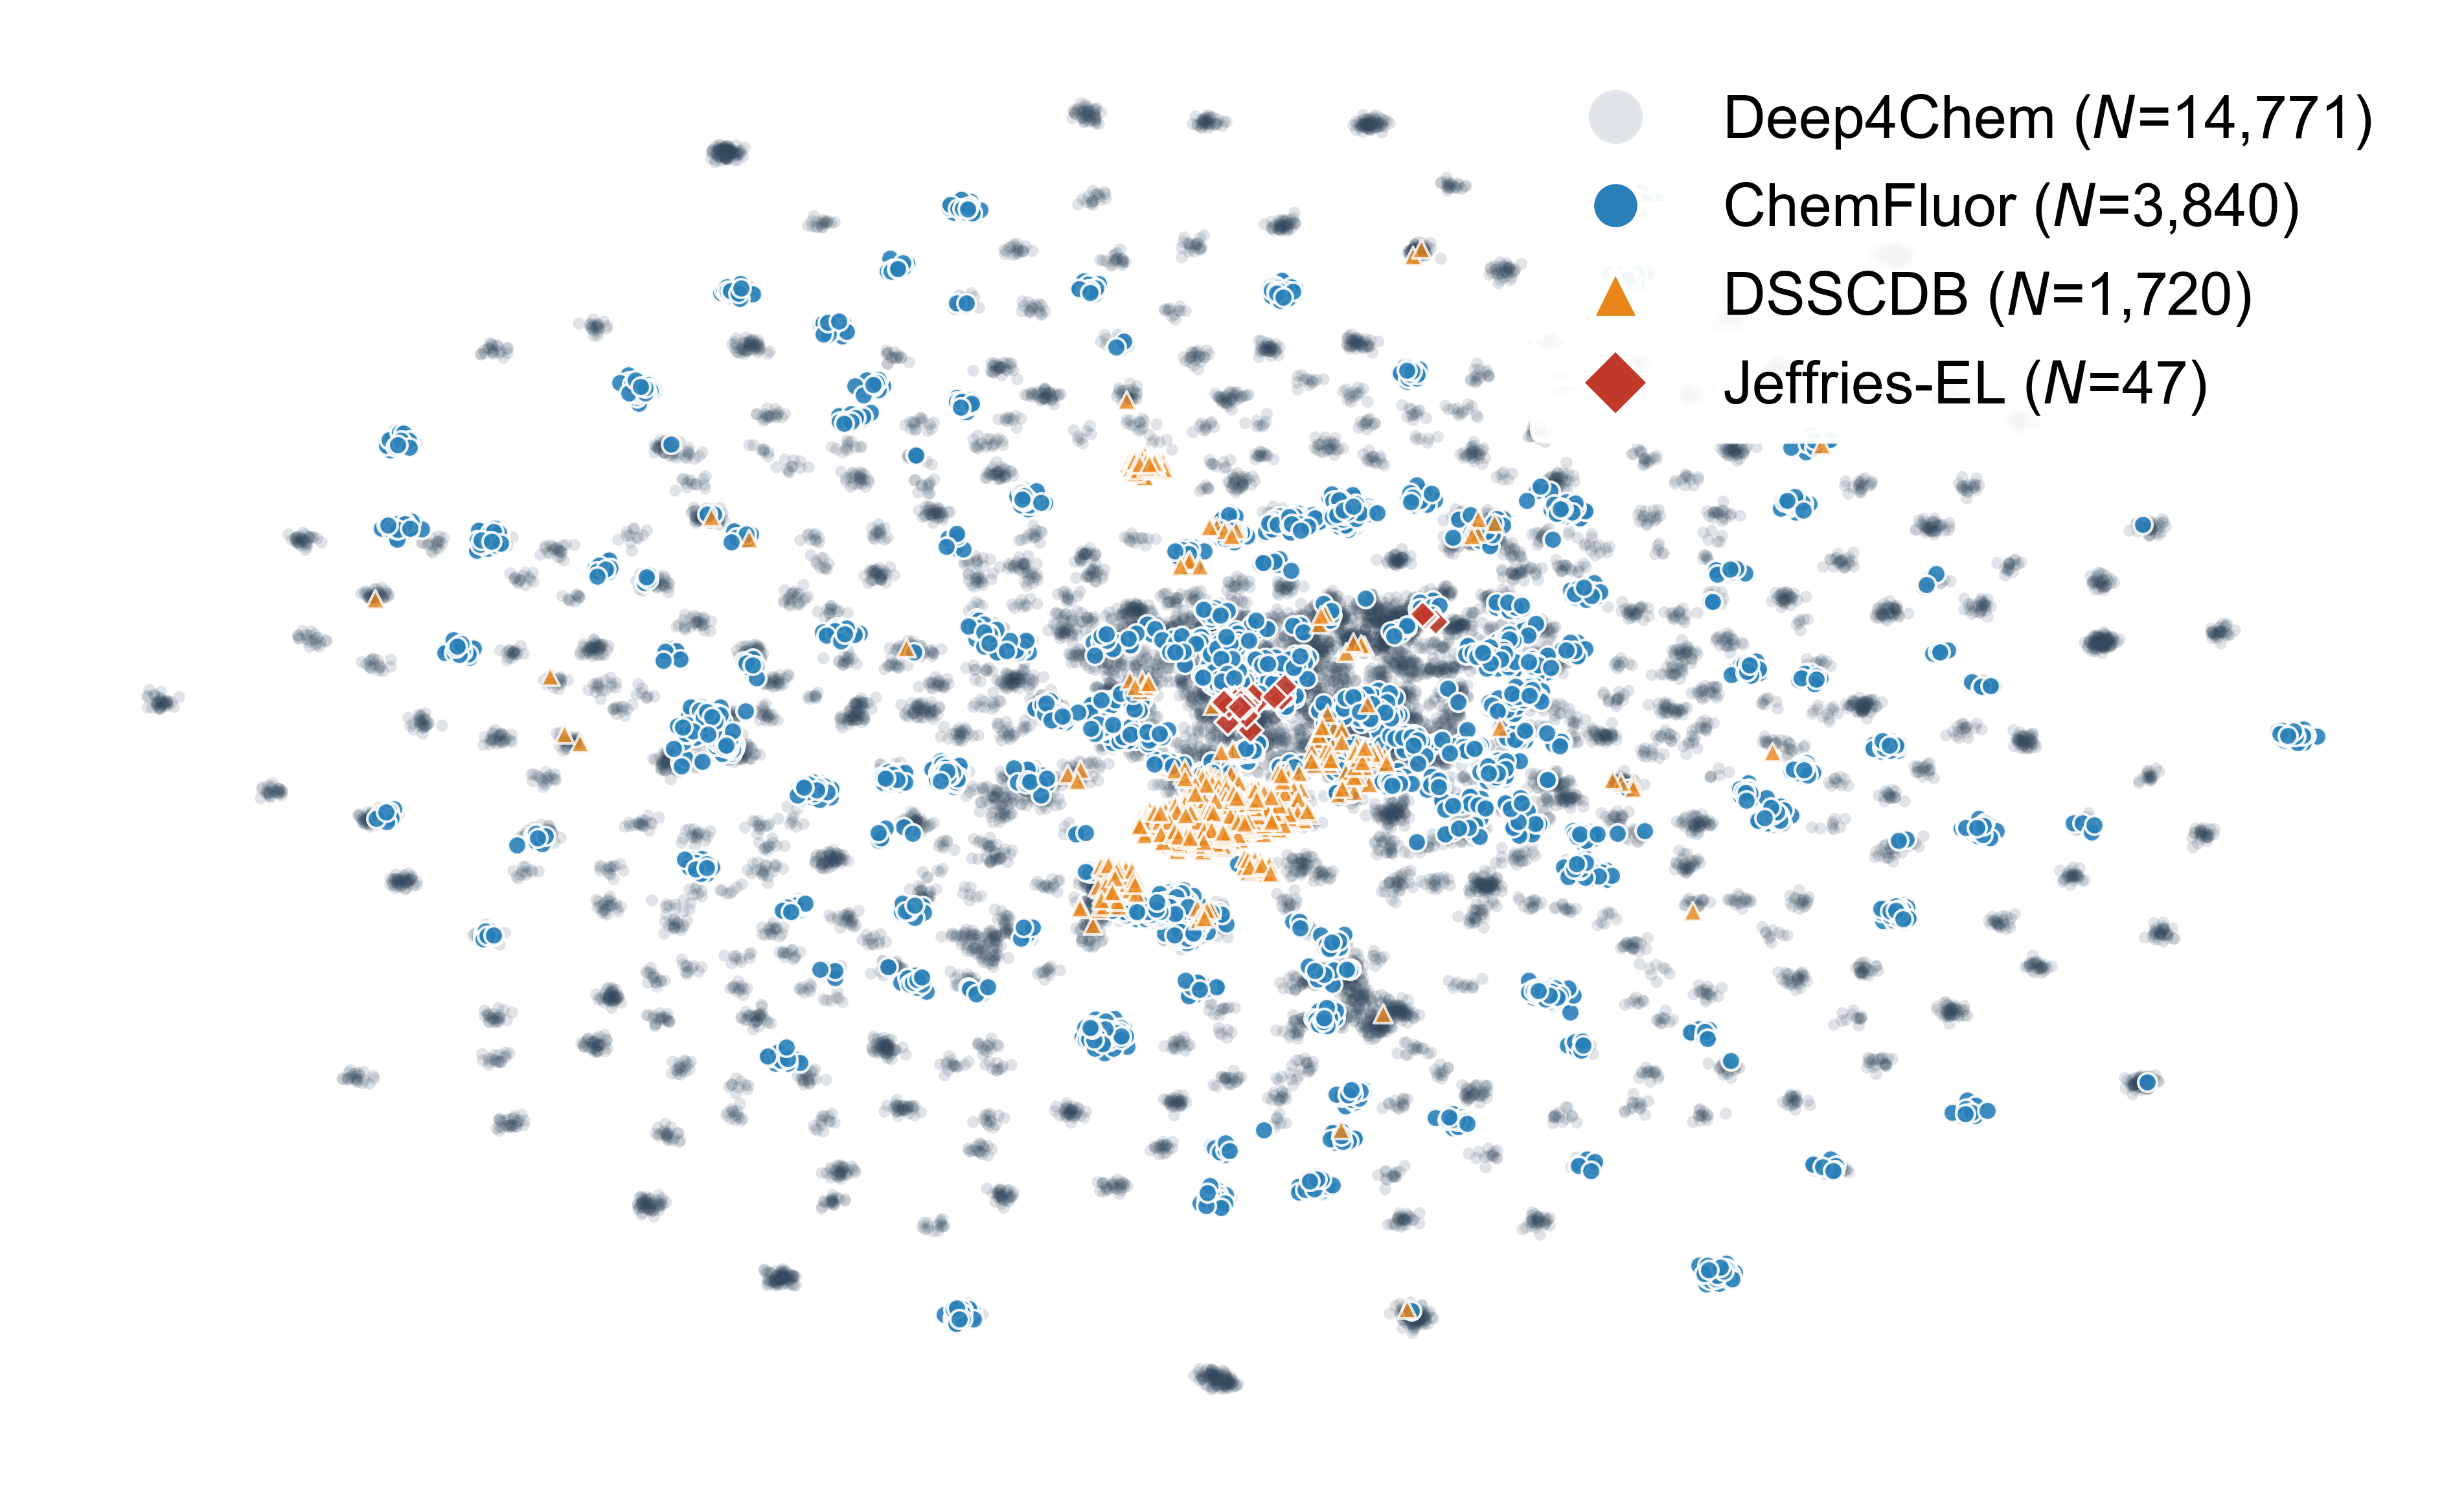
\includegraphics[width=0.9\linewidth]{figures/umap_pub_final.png}
  \caption{\textbf{Qualitative comparison of dataset chemical space.} Two-dimensional UMAP projection of molecules from all datasets computed from 2048-bit Morgan fingerprints (radius 2) using the Jaccard distance. To reduce overplotting due to repeated structures (e.g., identical fingerprints across solvents), points are displayed with a small random jitter.}
  \label{fig:umap_pub_final}
\end{figure}

All datasets were preprocessed following the protocol of Greenman \textit{et al.}~\cite{greenman2022multi} without modification. Molecular structures were canonicalized using RDKit, and only solution-phase measurements were retained; solid-state measurements were excluded. For molecules with multiple reported measurements in the same solvent, entries were filtered based on consistency: measurements differing by more than 5~nm were discarded, while remaining duplicate measurements were averaged. Measurements corresponding to the same molecular structure in different solvents were treated as distinct datapoints through solvent-specific feature representations. 

For datasets containing both absorption and emission measurements, the number of usable datapoints differs between targets due to incomplete experimental coverage. All analyses were therefore conducted on target-specific subsets derived from the same underlying molecular pool. Unless otherwise noted, dataset sizes $N$ refer to datapoints rather than unique molecules. A summary of dataset sizes and target availability is provided in Table~\ref{tab:datasets}.


\begin{table}[ht]
\centering
\caption{Summary of datasets used for optical property prediction after preprocessing.
Counts are reported as Absorption / Emission where applicable.}
\label{tab:datasets}
\begin{tabular}{l l c c}
\toprule
\textbf{Dataset} 
& \textbf{Target(s)} 
& \textbf{Datapoints} 
& \textbf{Unique Molecules} \\
\midrule
Deep4Chem 
& Abs., Emis. 
& 14{,}771 / 14{,}378 
& 5{,}841 / 5{,}597 \\

DSSCDB 
& Abs., Emis. 
& 1{,}720 / 690 
& 1{,}647 / 674 \\

ChemFluor 
& Abs., Emis. 
& 3{,}840 / 3{,}953 
& 2{,}622 / 2{,}617 \\

Jeffries-EL 
& Emis. 
& 47 
& 47 \\
\bottomrule
\end{tabular}
\end{table}

\subsection{Data Splitting and Training Regimes}

To assess generalization under both interpolation and distribution shift, we employ two splitting strategies. Random splits are used to approximate in-distribution generalization, while Bemis--Murcko scaffold splits are used to evaluate extrapolation to unseen chemical scaffolds. We adopt the same random and Bemis--Murcko scaffold splitting procedures as Greenman \textit{et al.}~\cite{greenman2022multi} and verify split equivalence by matching scaffold assignments and split indices.
To quantify the effective degree of distribution shift induced by each splitting strategy, we compute the maximum test-to-train Tanimoto similarity for all test molecules under both random and scaffold splits (Figure~\ref{fig:split-validation}). As expected, scaffold splitting substantially reduces train–test chemical overlap for Deep4Chem and ChemFluor, while DSSCDB exhibits comparatively high similarity even under scaffold splits, consistent with its narrower chemical diversity.

\begin{figure*}[t]
  \centering
  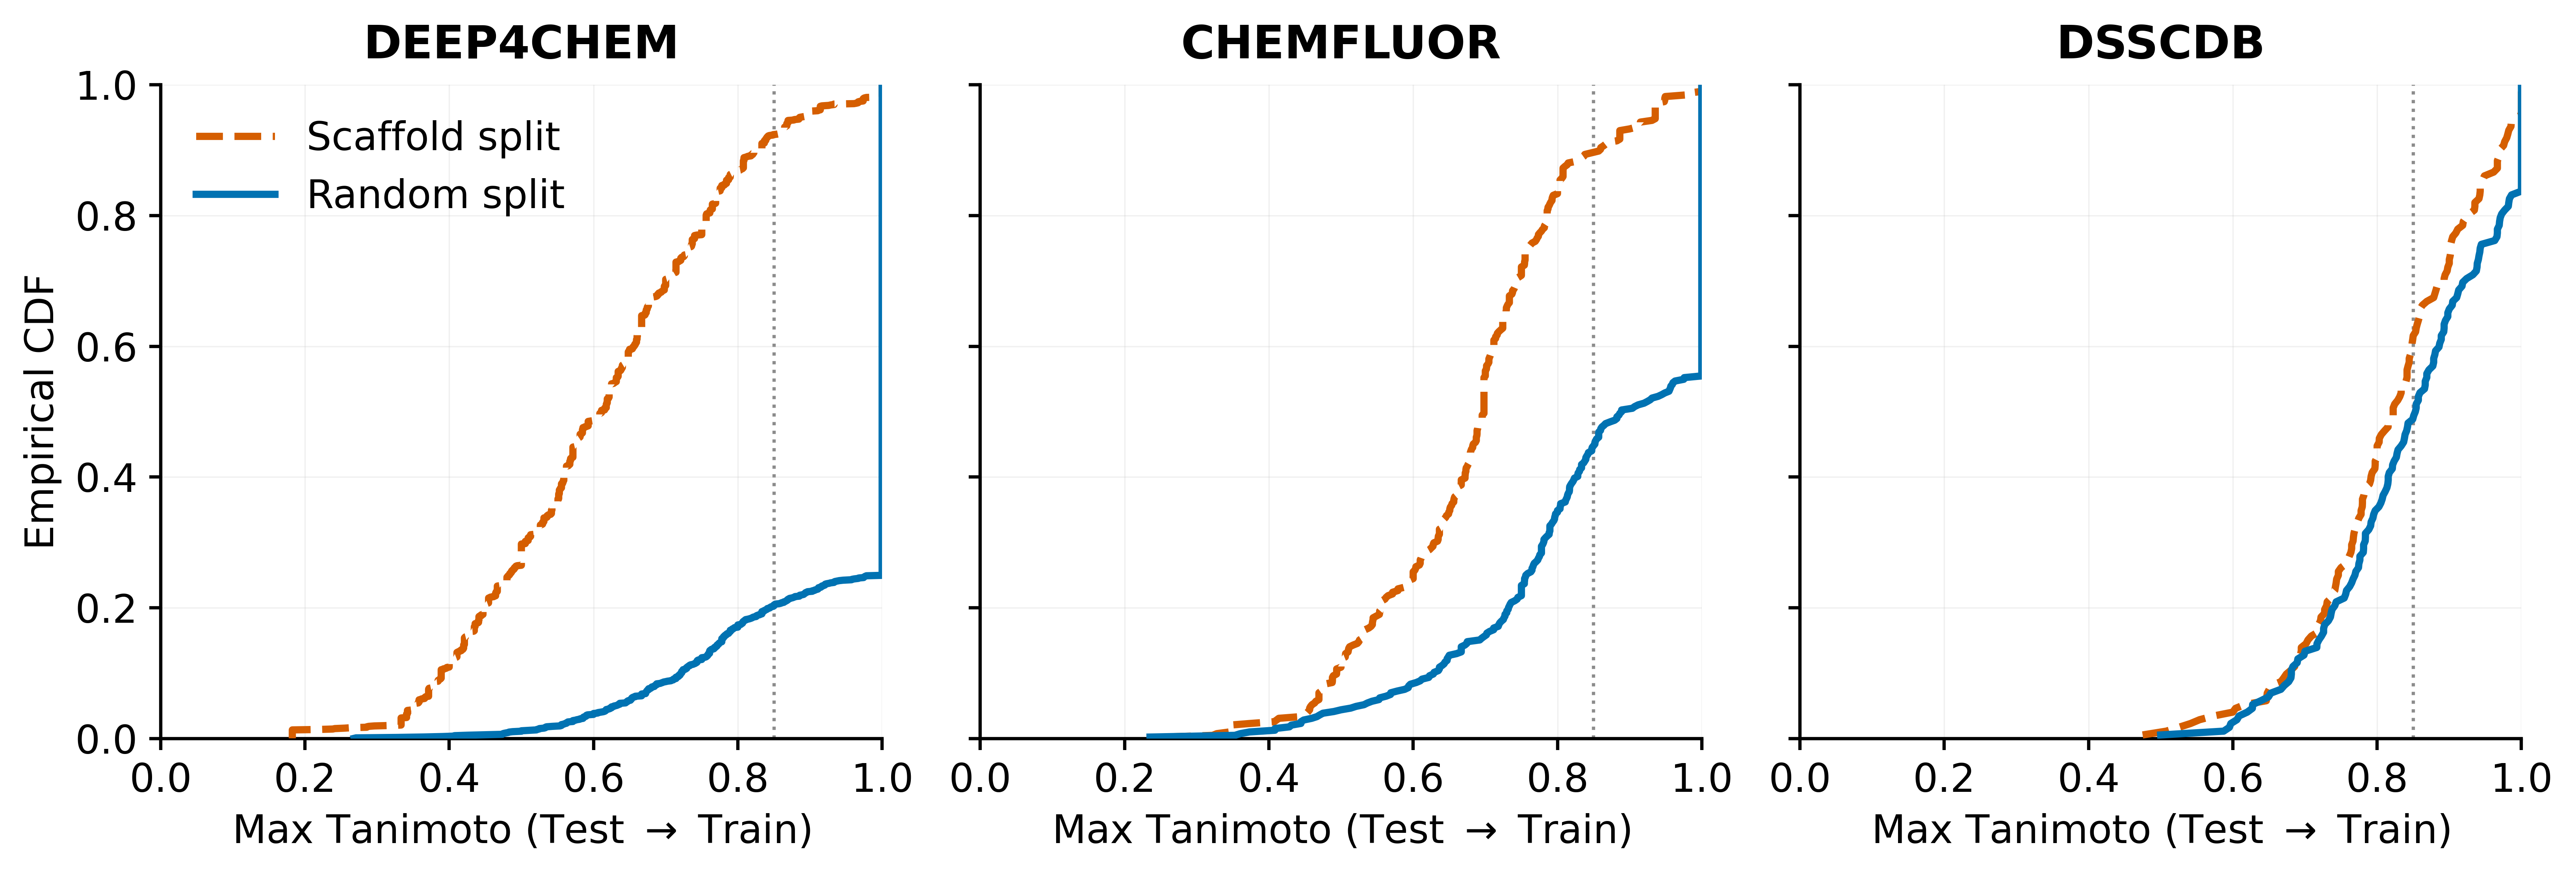
\includegraphics[width=0.9\linewidth]{figures/split_validation_cdf.png}
  \caption{\textbf{Train–test chemical similarity under random and scaffold splits.}
Empirical cumulative distribution functions (CDFs) of the maximum Tanimoto similarity between each test molecule and the training set, computed using Morgan fingerprints, for random and Bemis--Murcko scaffold splits across Deep4Chem, ChemFluor, and DSSCDB.
Vertical dotted lines indicate a commonly used similarity threshold ($T=0.85$), above which molecules are typically considered highly similar.
Scaffold splits substantially reduce train–test chemical overlap for Deep4Chem and ChemFluor, while DSSCDB exhibits higher intrinsic similarity across splits, reflecting its more chemically homogeneous composition.}

  \label{fig:split-validation}
\end{figure*}

\paragraph{Fixed subsampling for data-regime experiments.}
To evaluate performance as a function of training set size $N$, we constructed fixed subsampled training sets from each canonical split. For a given dataset, target, and split type, the original validation and test sets were held fixed, and training subsets were generated by sampling without replacement from the canonical training pool at sizes $N \in \{50,100,250,1000,4000\}$, as well as the full training set where available. For datasets with smaller training pools, only the feasible subset sizes were considered. Subsampling was performed using a fixed random seed, and the same subsampled training sets were reused across all model architectures and random initialization runs to ensure that differences across $N$ reflect model behaviour rather than variation in the sampled training examples. For hybrid models, downstream heads were trained on embeddings extracted from the corresponding subsampled training set, with validation and test evaluation performed on the fixed canonical splits. 


\subsection{Model Training Protocols}

\paragraph{End-to-end D-MPNN training.}
For each data regime, we conducted a 200-trial Optuna Bayesian hyperparameter search over architectural and optimization parameters, including network depth, FFN capacity, dropout rate, batch size, and learning-rate schedule. Optimization was performed using the Adam optimizer with a learning-rate warmup schedule and mean squared error (MSE) loss. We fixed the hidden dimension of the encoder at 482, consistent with Greenman \textit{et al.}~\cite{greenman2022multi} to ensure a consistent representational capacity across all data regimes and to mitigate numerical instability observed in ultra-small $N$ settings when the hidden dimension was allowed to vary.

Unless explicitly tuned, all remaining parameters were set to Chemprop defaults. Models were trained for a fixed 200 epochs without early stopping. This protocol was chosen to strictly isolate the impact of dataset size on training dynamics, avoiding the confounding influence of varying stopping criteria across data regimes. For each data regime, the optimal hyperparameter configuration identified by Optuna was reused across all ensemble members. To verify that fixed training horizons do not induce late-stage overfitting, we inspected training and validation trajectories across representative small- and large-data regimes and observed stable convergence without divergence in validation error (see Figure~\ref{fig:si-convergence}).

\paragraph{Hybrid model training.}
For the hybrid paradigm, D-MPNN encoders were pretrained as described above, then frozen. The downstream XGBoost heads were tuned via a separate 100-trial Optuna search for each $N$, optimizing tree depth, learning rate ($\eta$), and regularization terms ($\lambda, \alpha$).

\paragraph{Ensembling and Reproducibility.}
To mitigate stochasticity arising from random initialization and training dynamics, all reported performance metrics are based on ensemble predictions unless otherwise noted.
\begin{itemize}
\item \textbf{Deep and Hybrid Models:} Ensembles consist of $M=5$ independently trained models (distinct random seeds) sharing the same hyperparameter configuration. For hybrid models, this involves pairing 5 independently trained encoders with 5 corresponding downstream heads.
\item \textbf{Gradient-Boosted Baselines:} Due to their low computational cost, tree-based baselines are evaluated using larger ensembles of $M = 30$ models. 
\end{itemize}

\subsection{Evaluation Metrics}

Model performance is evaluated using Root Mean Squared Error (RMSE) computed on the held-out test set. All reported results correspond to the RMSE of the ensemble-averaged prediction. Where shown, error bars denote 95\% percentile bootstrap confidence intervals for the test RMSE, computed by resampling test molecules with replacement (2000 replicates). These intervals reflect sampling variability of the evaluation set and do not quantify variability across random initializations or ensemble members.


All deep learning models were implemented using PyTorch (v1.12) within the Chemprop framework (v1.6.1)~\cite{yang2019analyzing}. Chemical informatics operations and featurization were performed using RDKit (v2022.03.1), and gradient-boosted tree models were implemented using XGBoost (v1.6.2). Training and evaluation were conducted on NVIDIA H100 GPUs.

To ensure reproducibility, all code, canonical data splits, and trained model checkpoints used in this thesis are available at \url{https://github.com/michaelmontemurri/uvvis-hybrid-gnn}.


\section{Results and Discussion}
\subsection{Absorption Wavelength Prediction Across Data Regimes}
% ------------------------------------------------------------------
% Absorption: multi-panel comparison across datasets
% ------------------------------------------------------------------
\begin{figure*}[t]
  \centering
  \includegraphics[width=0.8\linewidth]{figures/abs_multipanel_bootstrap_ci.png}
  \caption{\textbf{Peak absorption wavelength ($\lambda_{\max}$) prediction across Deep4Chem, ChemFluor, and DSSCDB.} Test RMSE versus training set size $N$ for random (top row) and Bemis--Murcko scaffold (bottom row) splits. Each column corresponds to a dataset and uses dataset-specific $N$ values. Error bars indicate 95\% percentile bootstrap confidence intervals for the test RMSE, computed by resampling test molecules with replacement (2000 replicates). Models marked with an asterisk incorporate TD-DFT–derived HOMO--LUMO gap information.}
  \label{fig:multipanel-n-vs-rmse}
\end{figure*}

\paragraph{Consistent hybrid advantage in low-to-mid data regimes.}
Figure~\ref{fig:multipanel-n-vs-rmse} reports test RMSE as a function of training set size $N$ for peak absorption wavelength ($\lambda_{\max}$) prediction. Across datasets and split types, the hybrid D-MPNN$\rightarrow$XGBoost model generally outperforms the end-to-end D-MPNN in low-to-mid data regimes ($N \leq 1000$), with the strongest gains appearing under scaffold splits and in the smaller training-size settings. The magnitude of this effect is summarized in Table~\ref{tab:hybrid_pct_improvement}; for Deep4Chem, we observe an average RMSE reduction of \textbf{6.5\% for random splits} and \textbf{9.2\% for scaffold splits} within the $50 \leq N \leq 1000$ range.

We attribute this overall advantage to the structural regularization of gradient-boosted trees. In data-limited regimes, high-dimensional FFN heads are prone to high-variance estimation and overfitting. In contrast, the tree-based structure of XGBoost enforces simpler decision boundaries within the learned embedding space, acting as a robust regularization prior. This effect is most pronounced under scaffold splits (Deep4Chem), where the distribution shift is largest (see Figure~\ref{fig:split-validation}). As data availability increases ($N > 1000$) or distribution shift decreases (DSSCDB), the end-to-end model receives sufficient signal to stabilize the head, and the performance gap closes.


\begin{table}[h]
\centering
\caption{Percentage RMSE improvement of the Hybrid model (frozen D-MPNN embeddings $\rightarrow$ XGBoost) relative to the end-to-end D-MPNN. Positive values indicate lower RMSE for the Hybrid model.}
\label{tab:hybrid_pct_improvement}
\begin{tabular}{lcccccc}
\toprule
 & \multicolumn{2}{c}{\textbf{DEEP4CHEM}} & \multicolumn{2}{c}{\textbf{CHEMFLUOR}} & \multicolumn{2}{c}{\textbf{DSSCDB}} \\
\cmidrule(lr){2-3} \cmidrule(lr){4-5} \cmidrule(lr){6-7}
$N$ 
& Rand (\%) & Scaf (\%) 
& Rand (\%) & Scaf (\%) 
& Rand (\%) & Scaf (\%) \\
\midrule
50   & \textbf{+5.7} & \textbf{+7.7} & \textbf{+10.8} & \textbf{+9.8}  & \textcolor{gray}{-1.6} & \textbf{+5.4} \\
100  & \textbf{+8.8} & \textbf{+10.6}& \textbf{+9.8}  & \textbf{+15.6} & \textbf{+2.8} & \textbf{+3.5} \\
250  & \textbf{+7.5} & \textbf{+7.6} & \textbf{+8.0}  & \textbf{+6.0}  & \textbf{+2.7} & \textbf{+3.5} \\
1000 & \textbf{+4.1} & \textbf{+11.0}& +1.2           & \textbf{+5.4}  & \textbf{+5.4} & +0.4 \\
Max $N^{\dagger}$ 
     & \textbf{+8.0} & +1.3           & +0.8           & \textcolor{gray}{-28.8} & \textbf{+9.3} & \textbf{+7.0} \\
\bottomrule
\multicolumn{7}{l}{\footnotesize $^\dagger$ Max $N$: DEEP4CHEM (11,816), CHEMFLUOR (3,072), DSSCDB (1,376).}
\end{tabular}
\end{table}

\paragraph{Benchmarking against physical and classical baselines.}
Fingerprint-based baselines exhibit the expected hierarchy: augmenting Morgan fingerprints with physicochemical descriptors improves performance, but both graph-based models (End-to-End and Hybrid) generally outperform these fixed-feature approaches once $N \geq 250$.

In the ultra-low data regime ($N \leq 100$), physics-informed baselines utilizing TD-DFT--derived HOMO--LUMO gaps (dashed lines) remain the most robust, particularly under scaffold splits. This highlights the necessity of strong physical inductive biases when experimental supervision is scarce. However, as $N$ increases, the D-MPNN-based models rapidly overtake the DFT-augmented baselines. This crossover indicates that the learned graph representations eventually capture higher-order structural information that exceeds the predictive content of a single vacuum-phase orbital gap. The graph models achieve this accuracy without the computational overhead of calculating DFT descriptors at inference time.

\paragraph{Comparison to Multi-Fidelity Frameworks.}
We benchmark our approach against the multi-fidelity D-MPNN ensemble of Greenman \textit{et al.}~\cite{greenman2022multi}. Using identical preprocessing and scaffold splits on Deep4Chem, our Hybrid model achieves a test RMSE (27.5~nm) comparable to their reported ChempropMultiFidelity result (27.47~nm).

The Greenman framework relies on auxiliary pretraining with TD-DFT excitation energies. Generating this auxiliary data for the $\sim$5,800 molecules in Deep4Chem requires an estimated $10^5$ core-hours of quantum-chemical calculations (RDKit $\rightarrow$ xTB $\rightarrow$ DFT $\rightarrow$ TD-DFT) (K. Greenman, personal communication, Feb 11, 2026). Our results demonstrate that such expensive pretraining may not be necessary for comparable performance on this benchmark. By using a hybrid architecture with implicit regularization, we achieve comparable accuracy using purely experimental supervision, without the need for a quantum-chemical pipeline.

\paragraph{Summary: Regime-dependent tradeoffs and practical workflows.}
These results reveal a clear regime-dependent tradeoff. In the data-scarce limits ($N \lesssim 1000$) typical of experimental screening, the hybrid architecture offers meaningful accuracy gains; as dataset size increases, this advantage diminishes and fully joint optimization becomes competitive.
The computational cost of fitting an XGBoost head on fixed embeddings is negligible compared to the cost of training the D-MPNN encoder itself. Consequently, given a trained D-MPNN, practitioners can extract the learned embeddings and fit a lightweight XGBoost head with virtually no overhead. This ensures optimal performance in the low-data limit without sacrificing the scalability of the end-to-end model as data grows.
We note that this hybrid advantage is most pronounced for absorption; as detailed in the Supporting Information, results for emission prediction were less systematic, consistent with the greater physical complexity of excited-state relaxation and solvent reorganization effects, which are harder to capture in a static representation.

\subsection{Variance Decomposition}

Figure~\ref{fig:multipanel-n-vs-rmse} shows that model hybridization is most beneficial in low-$N$ regimes; we next ask which sources of stochasticity drive this behaviour. We use the variance decomposition framework introduced in Methods to identify which sources of stochasticity dominate predictive performance across data regimes, and to explain the observed convergence of hybrid and end-to-end models at scale.

\paragraph{Head sensitivity and selection.}
To isolate variability attributable solely to the regression head, we evaluated three models (MLP, RF, and XGBoost) on a fixed, pretrained D-MPNN encoder. As shown in the Supporting Information (Figure~\ref{fig:fixed-model}), XGBoost typically provided the strongest mean performance with minimal variance, motivating its adoption as the standard head for the hybrid architecture used throughout this work.

\paragraph{Regime-dependent variance decomposition.}
Figure~\ref{fig:var-decomp} presents the variance decomposition on Deep4Chem as a function of training set size. In small-data regimes ($N \leq 250$), a substantial proportion of predictive variability ($\sim$20--30\%) is attributable to the downstream head. This implies that under limited supervision, the mapping from molecular representation to property is underdetermined; the choice of regression model and its optimization significantly impacts generalization.

\begin{figure}[ht]
  \centering
  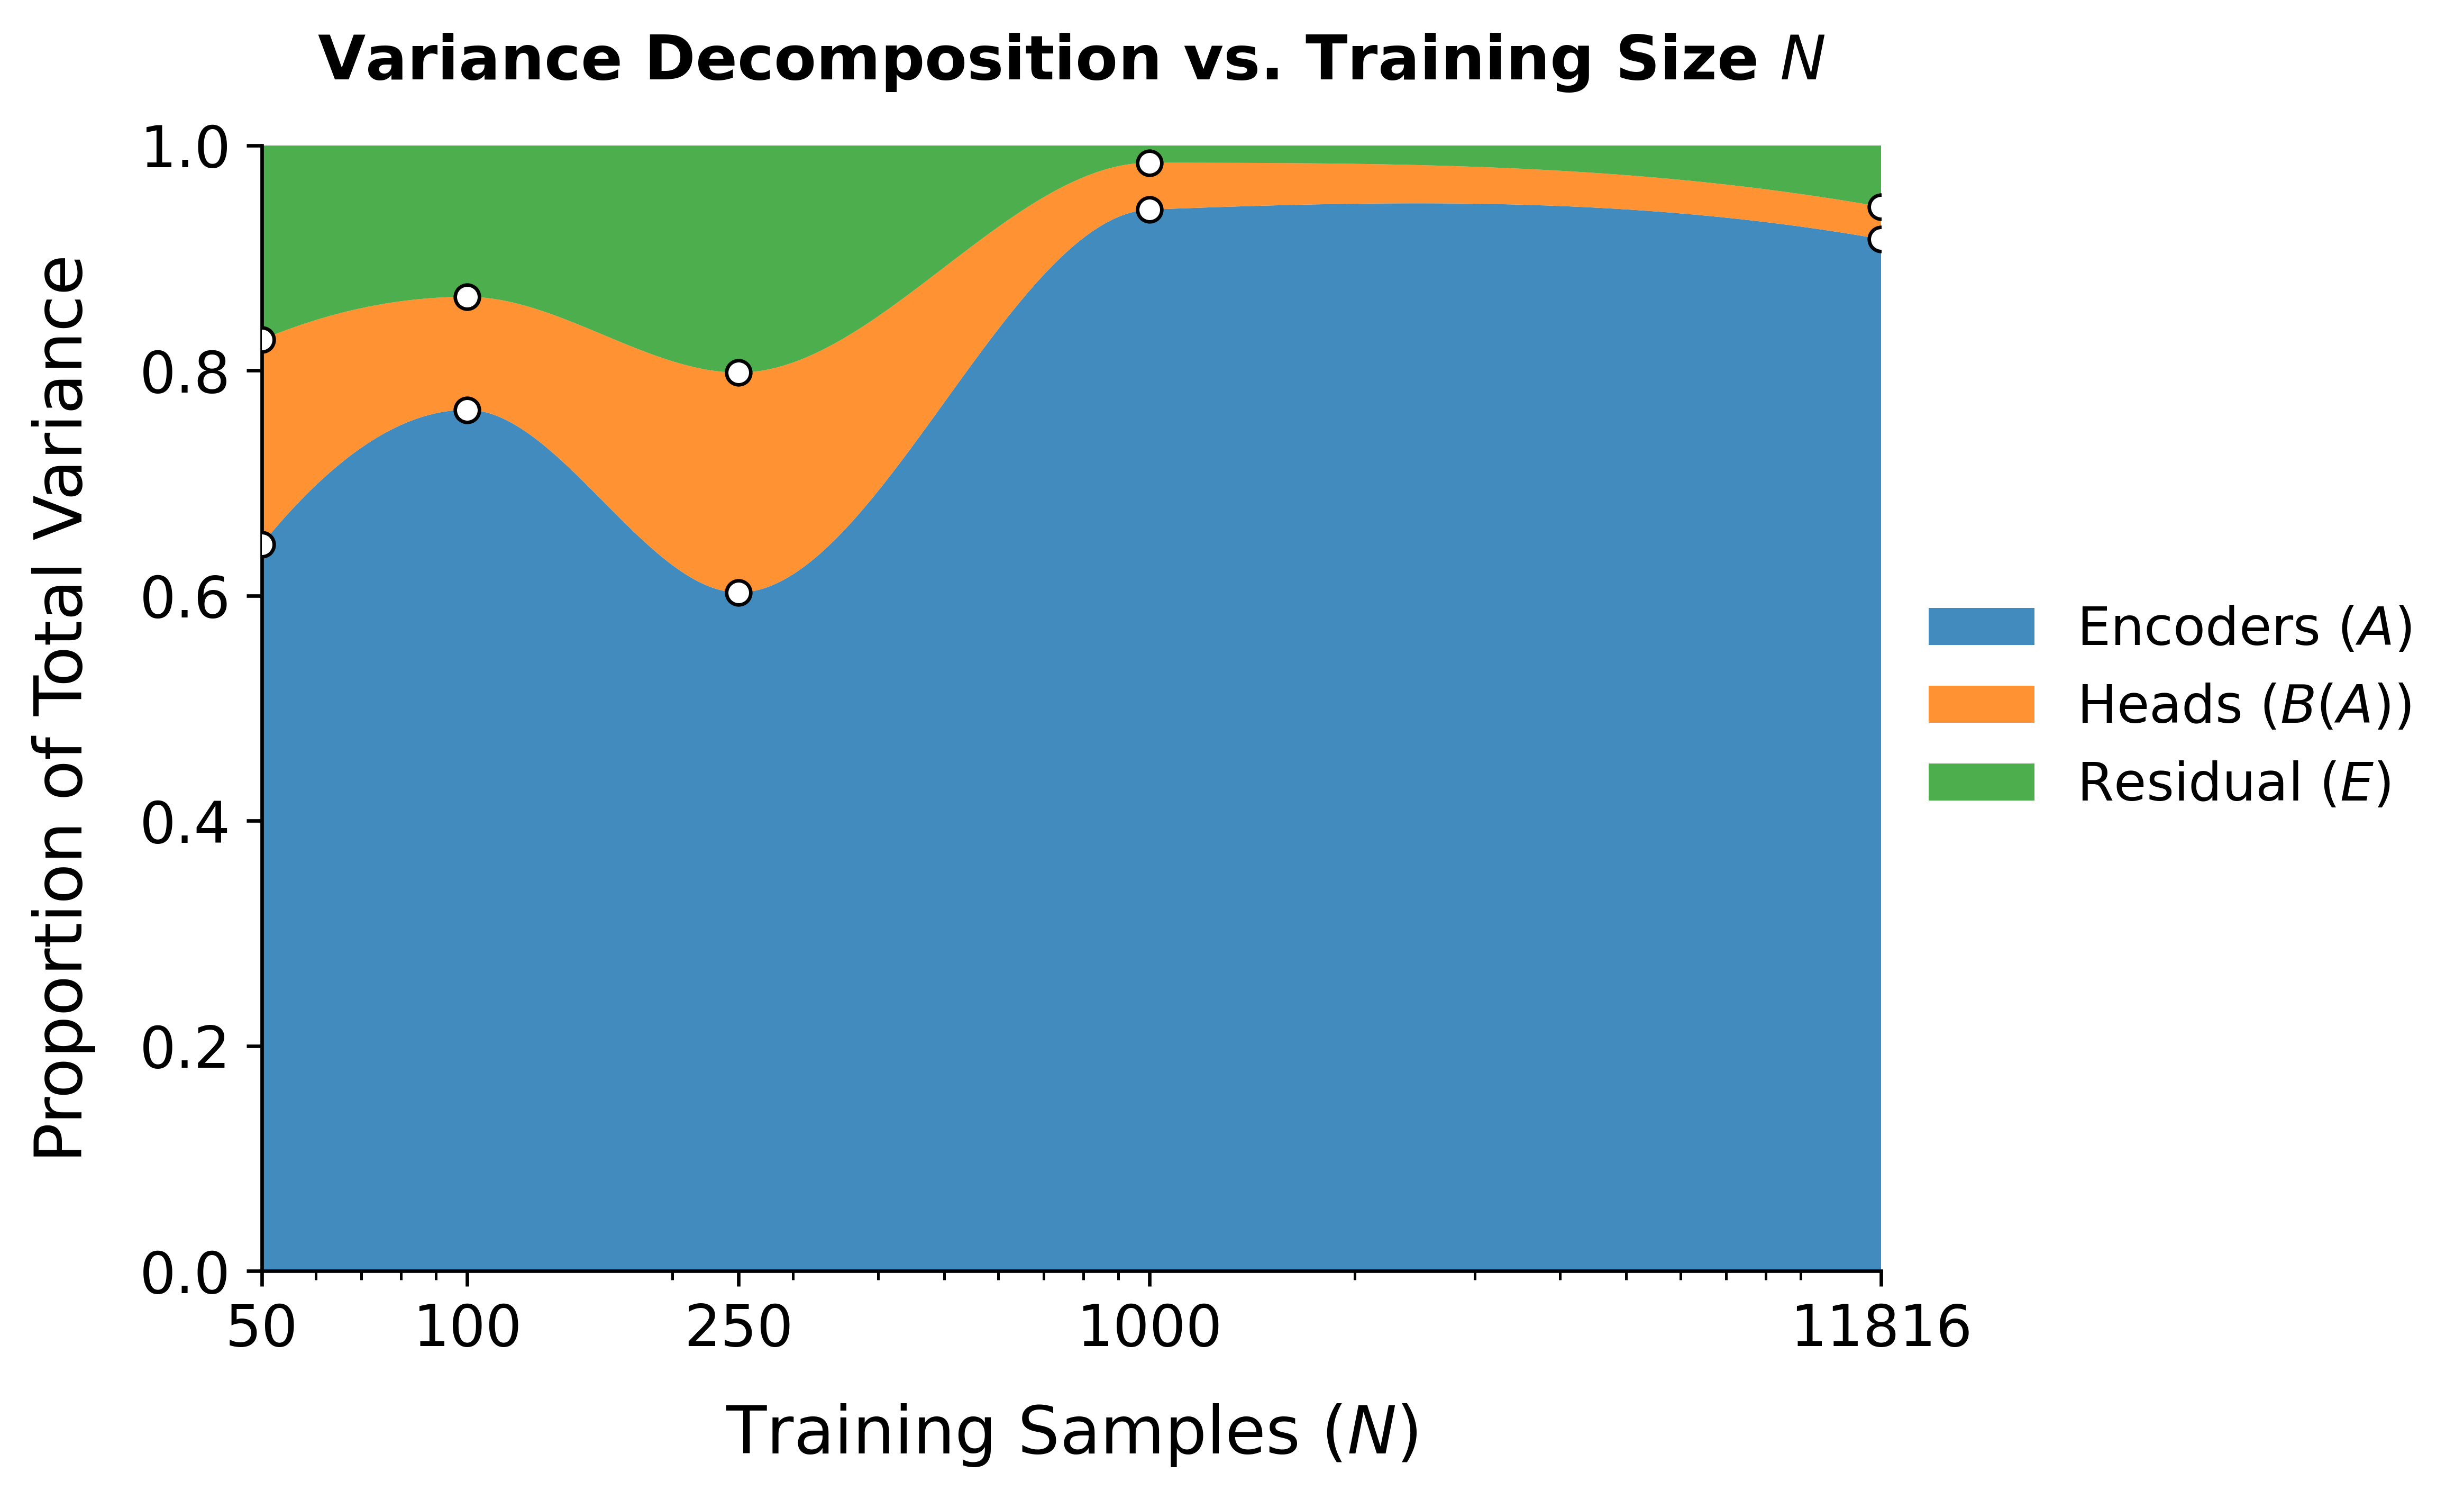
\includegraphics[width=0.9\linewidth]{figures/variance-decomp.png}
  \caption{\textbf{Proportion of total test-set RMSE variance attributable to encoder-level stochasticity, head-level variability, and residual noise.} The breakdown is shown as a function of training set size $N$ on Deep4Chem, with variance proportions estimated using a two-factor nested random-effects decomposition.}
  \label{fig:var-decomp}
\end{figure}

As $N$ increases, the contribution of the head diminishes, and predictive variability becomes dominated almost entirely by stochasticity in encoder training. This explains the convergence of hybrid and end-to-end models at scale: once the dataset is large enough to constrain the representation, the specific choice of head becomes less critical. The hybrid advantage in low-data regimes, therefore, stems from XGBoost's ability to efficiently navigate the high-variance ``head'' component of the error budget.

Uncertainty estimates for the variance components, obtained via bootstrap resampling, are reported in the Supporting Information (Table~\ref{tab:si_varcomp_bootstrap}); while confidence intervals are wide at small training set sizes, the qualitative dominance of encoder-level stochasticity is preserved across regimes.

\section{Transfer Learning and Pretraining Effects}
We next evaluate whether pretraining on the large Deep4Chem corpus can mitigate data scarcity in smaller, domain-specific tasks. We compare four strategies defined in Methods: Random Initialization, Zero-Shot Pretrained, Two-Stage Fine-Tuning, and Hybrid Transfer.

\begin{figure*}[t]
  \centering
  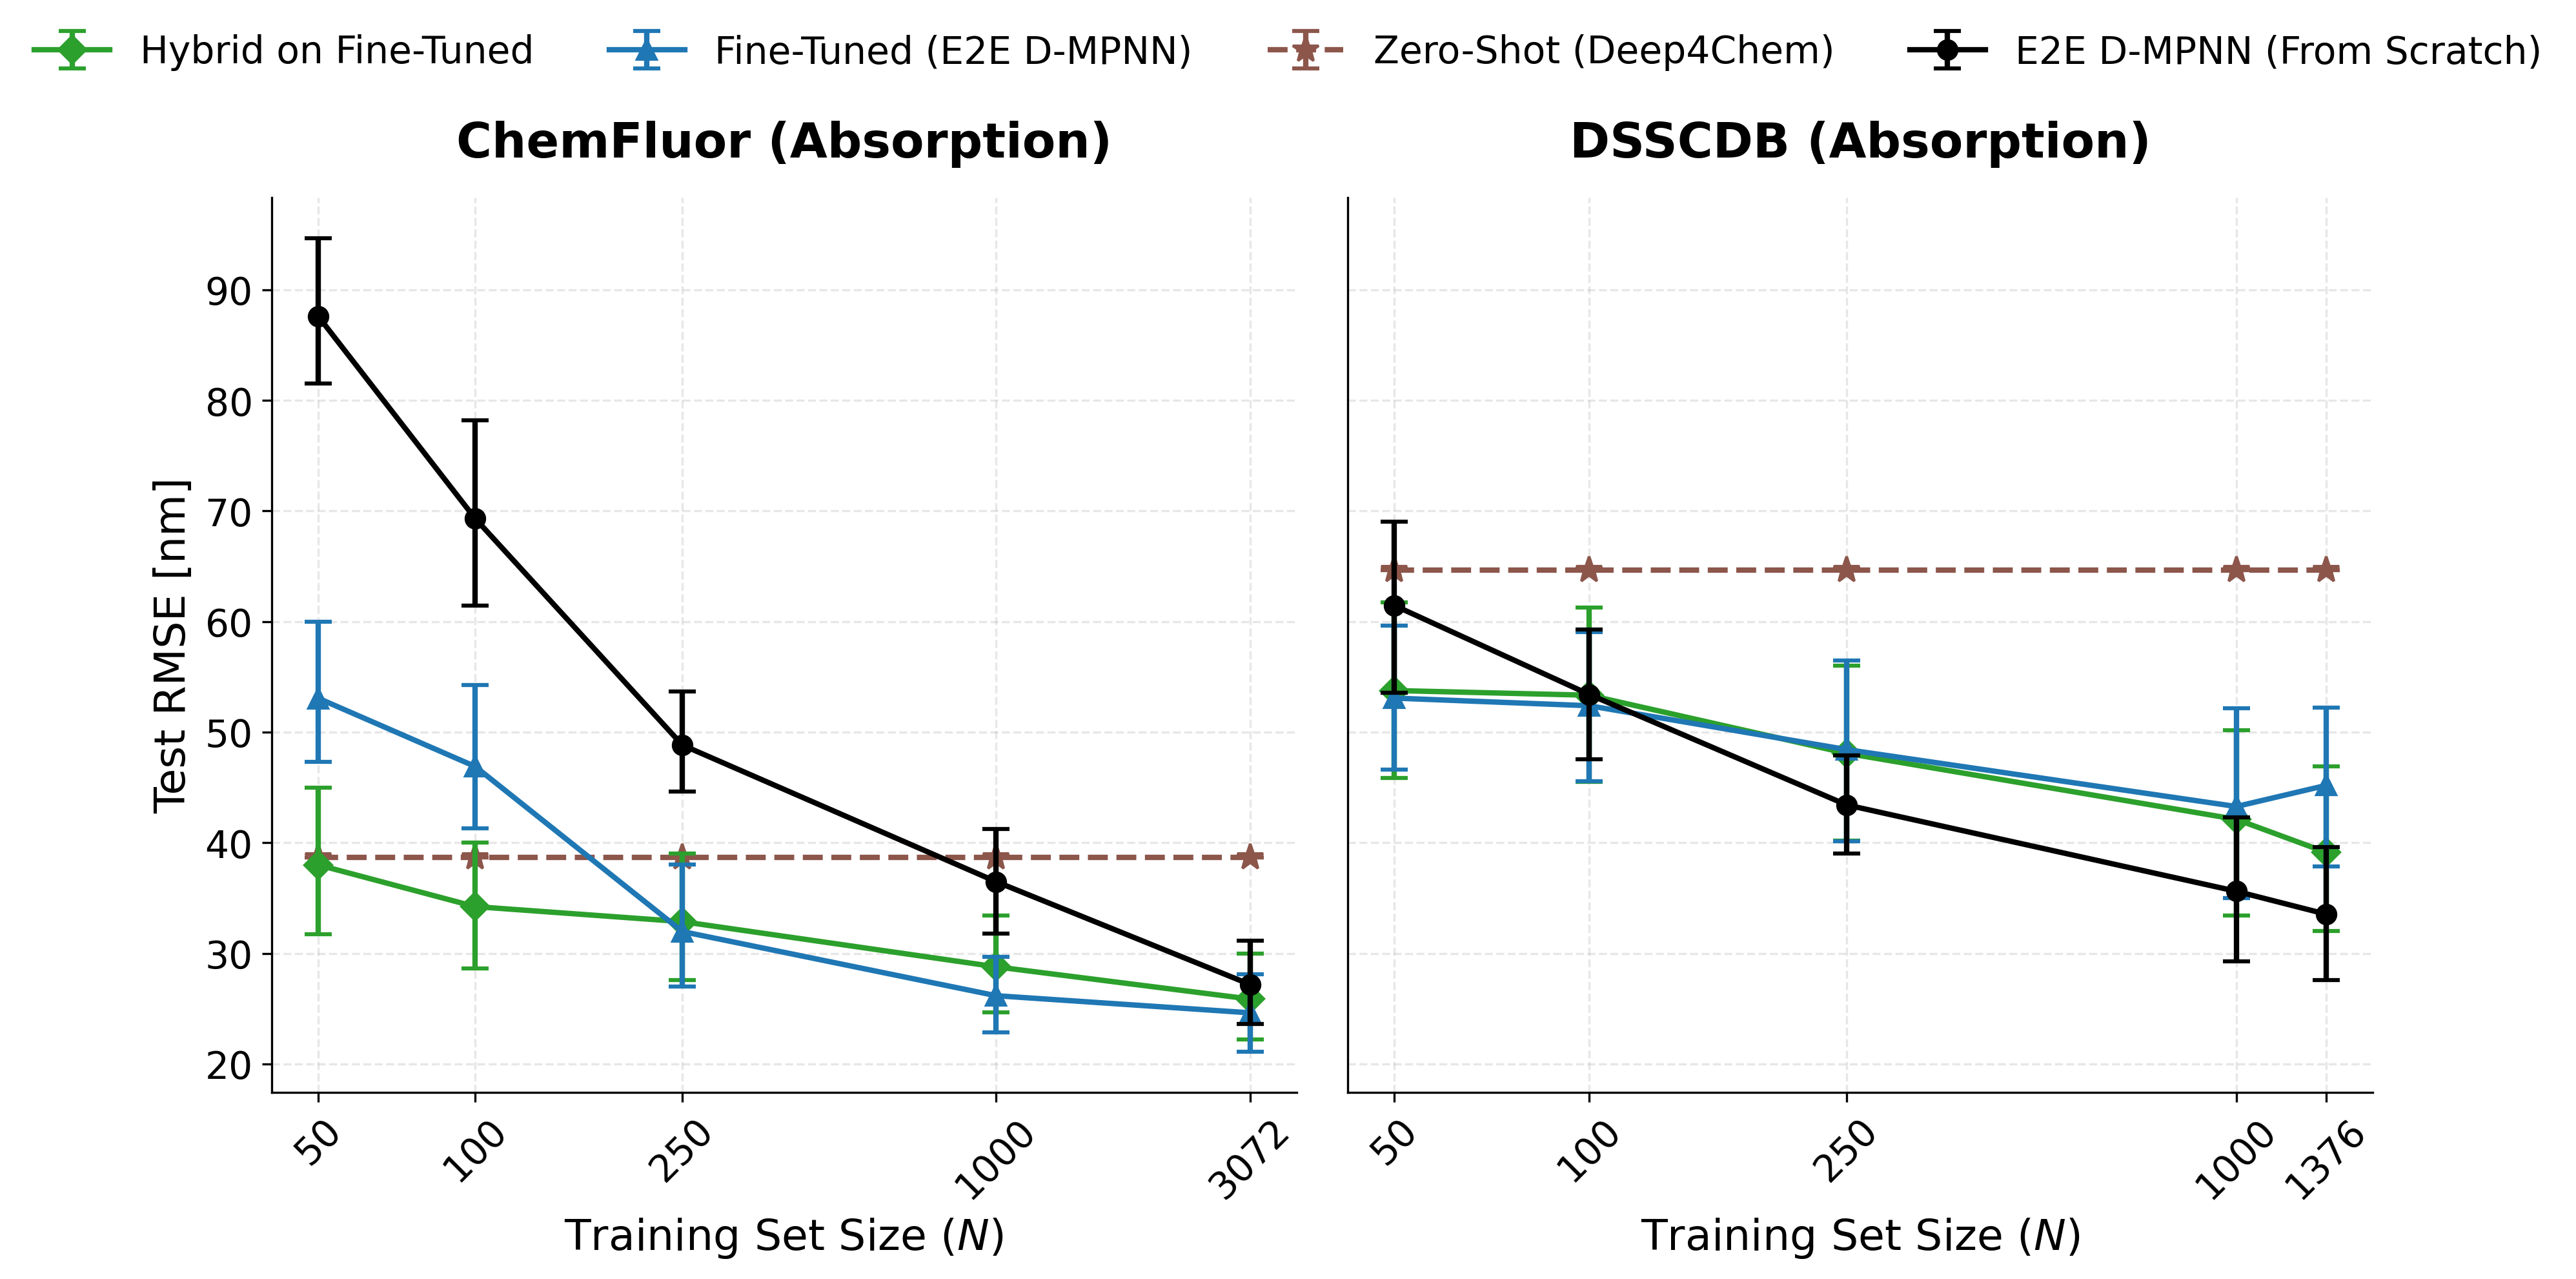
\includegraphics[width=0.9\linewidth]{figures/abs_transfer_multipanel_bootstrap.png}
  \caption{\textbf{Regime-dependent benefits of transfer learning.} 
  Test RMSE (scaffold split) versus training set size $N$ for \textbf{(A) ChemFluor} and \textbf{(B) DSSCDB}. 
  Strategies include training from scratch (black circles), two-stage fine-tuning of a Deep4Chem-pretrained encoder (blue triangles), and hybrid XGBoost head applied to fine-tuned embeddings (green diamonds). 
  The zero-shot performance of the Deep4Chem model (brown stars) is provided as a baseline. 
  Error bars indicate 95\% percentile bootstrap confidence intervals for the test RMSE, computed by resampling test molecules with replacement (2000 replicates).}
  \label{fig:transfer_multipanel}
\end{figure*}

\paragraph{Transfer to ChemFluor (High Chemical Overlap).}
Figure~\ref{fig:transfer_multipanel}A demonstrates that for ChemFluor, which shares significant structural similarity with Deep4Chem, transfer learning appears particularly effective. Fine-tuning a pretrained encoder yields substantial RMSE reductions over training from scratch in the $N \leq 1000$ regime. Notably, the Hybrid Transfer strategy on these fine-tuned embeddings provides even further improvement. This confirms that even when transfer is successful, the regularization benefits of the hybrid model persist in the ultra-low-data limit.

\paragraph{Transfer to DSSCDB (Low Chemical Overlap).}
In contrast, transfer to the DSSCDB dataset (Figure~\ref{fig:transfer_multipanel}B) illustrates the limitations of pretraining under distribution shift. DSSCDB contains distinct dye classes poorly represented in Deep4Chem. Consequently, the zero-shot baseline performs poorly, and fine-tuning offers only negligible gains at $N=50$. As data availability increases, models trained from scratch rapidly surpass the transfer-learning models. This likely reflects representational bias from pretraining.

\begin{figure}[t]
  \centering
  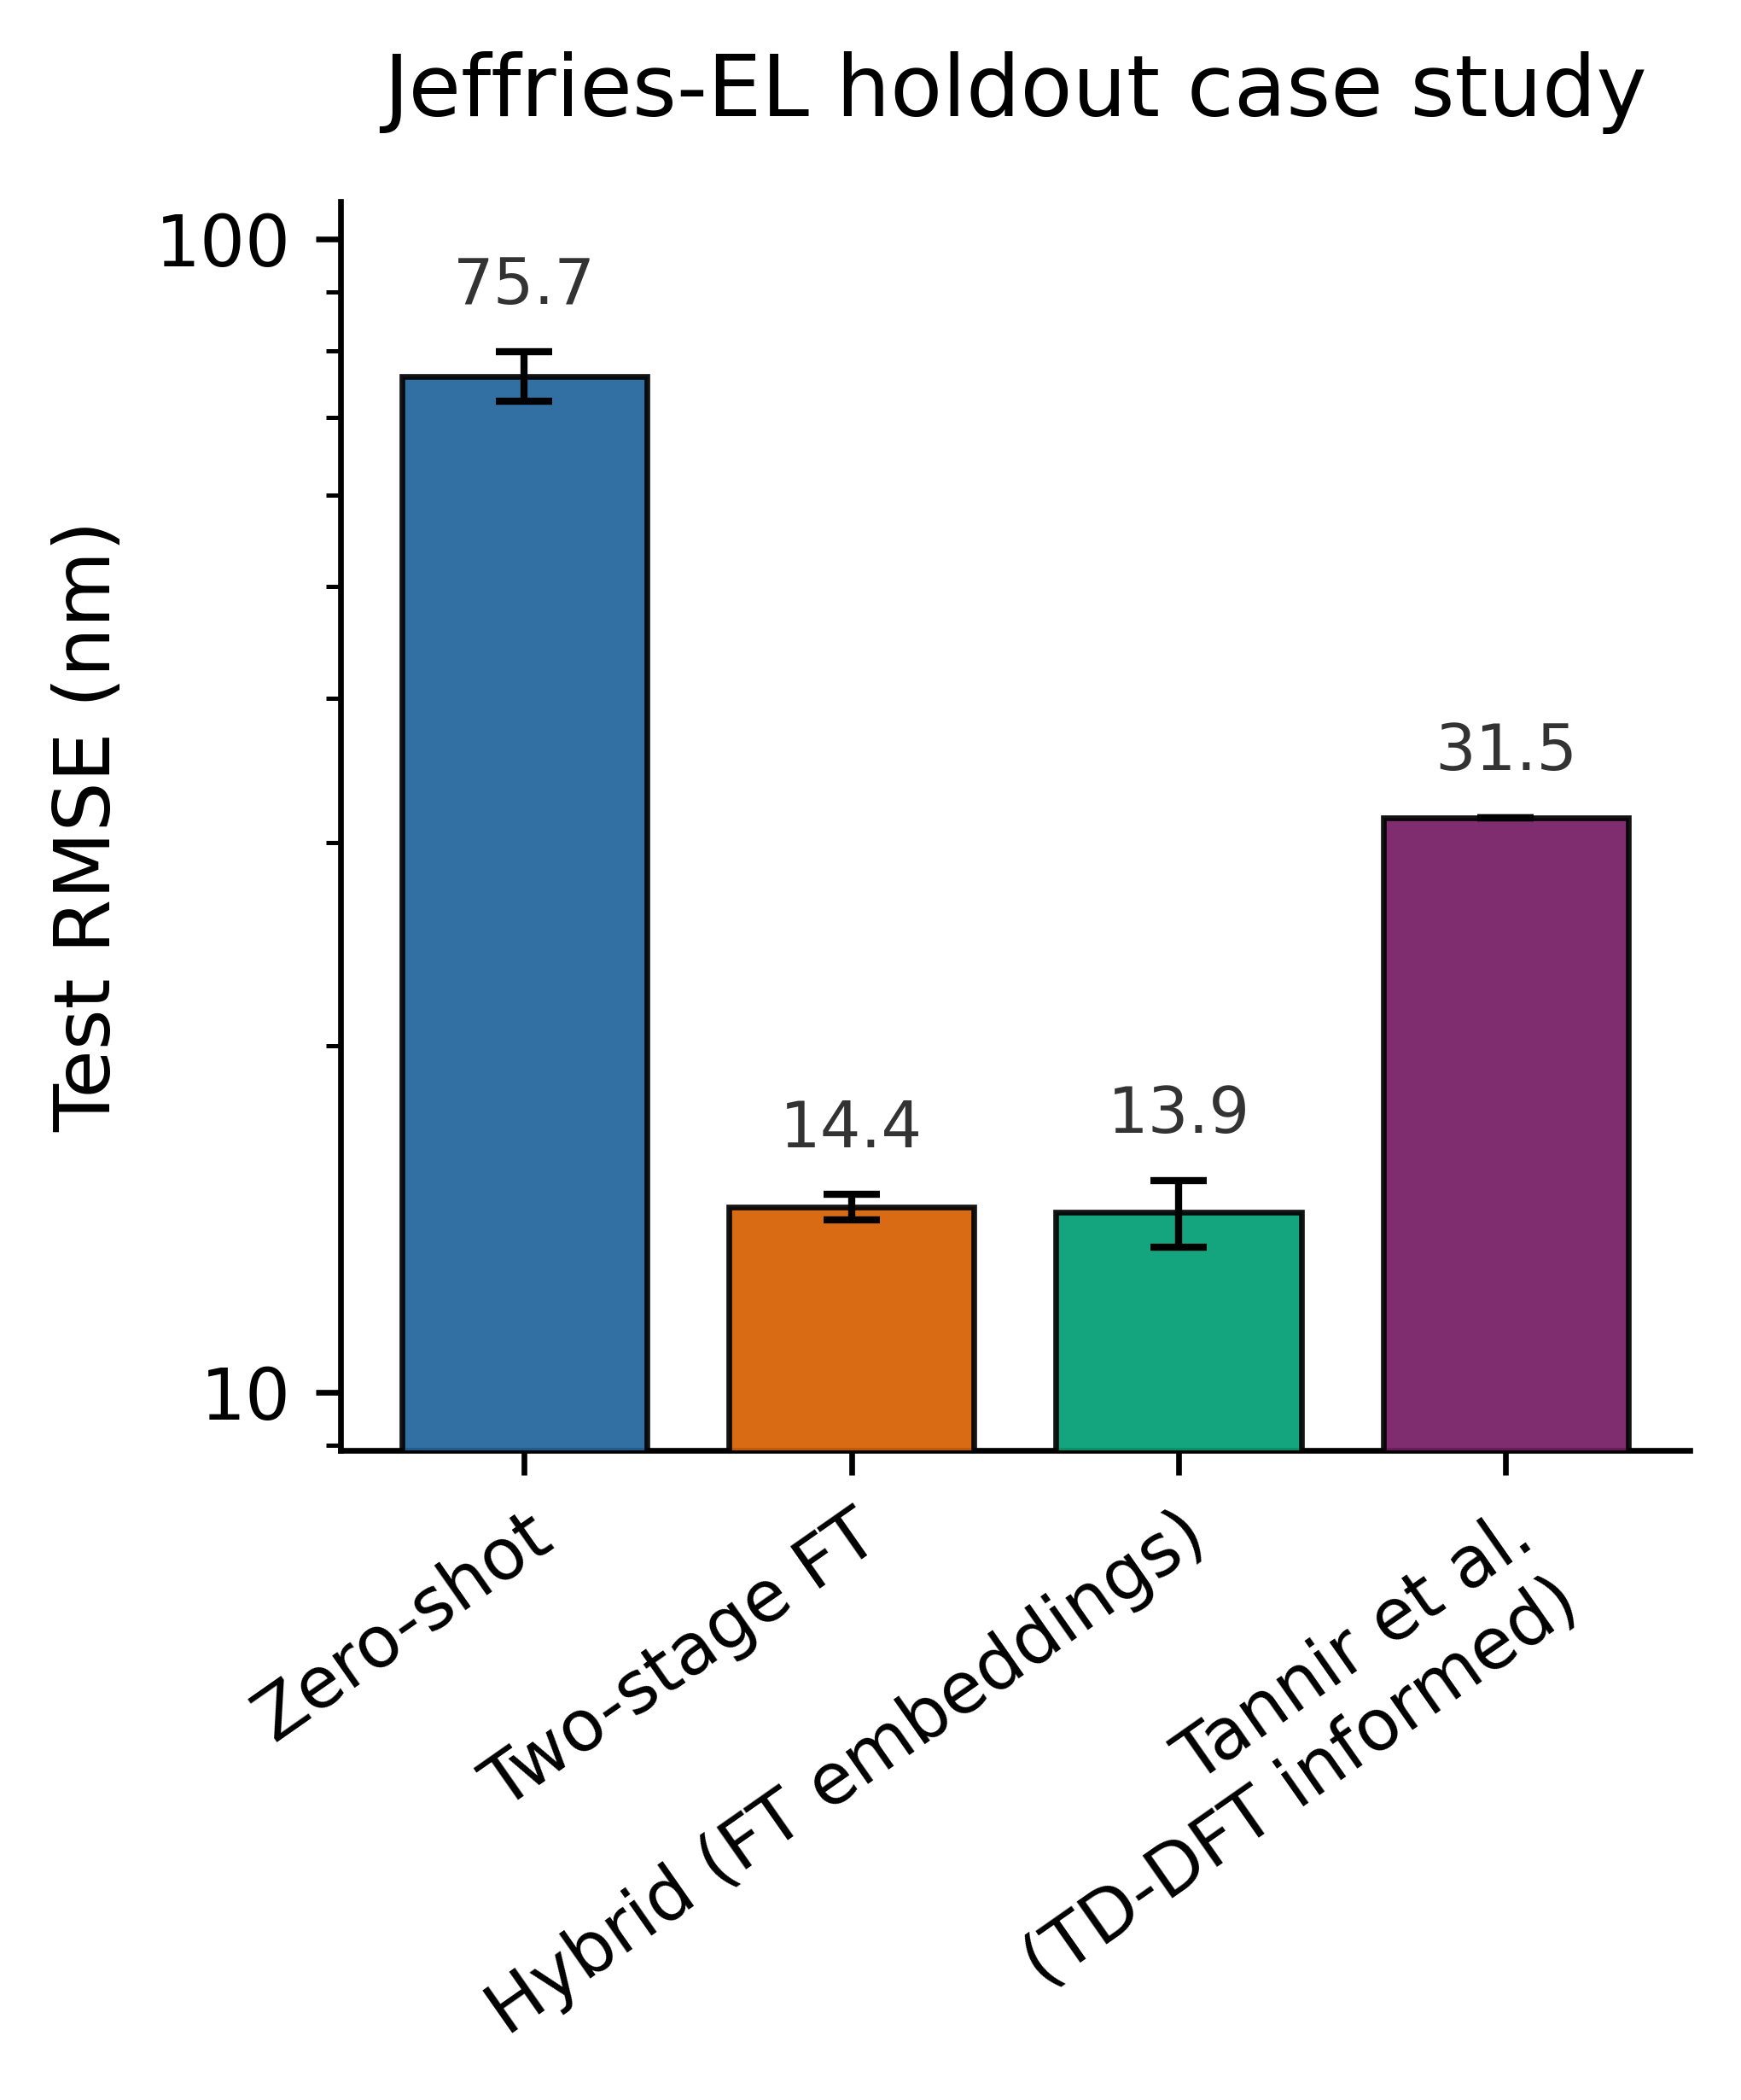
\includegraphics[width=0.5\linewidth]{figures/jeffries_case_study_bars.png}
  \caption{\textbf{Jeffries-EL Case Study ($N=43$).} Test RMSE on the holdout set. The Hybrid model trained on fine-tuned embeddings achieves the lowest error, outperforming both standard fine-tuning and domain-specific physics-informed baselines (Tannir \textit{et al.}).}
  \label{fig:jeffries_case_study}
\end{figure}

\paragraph{Case Study: Jeffries-EL (Ultra-Small $N$).}
Based on the transfer behaviours observed on ChemFluor and DSSCDB, we hypothesized that the Jeffries-EL dataset ($N=43$) would benefit significantly from pretraining due to its chemical alignment with Deep4Chem. Moreover, we anticipated that the hybrid architecture would further enhance performance by stabilizing the head in this ultra-low-data limit. The results are consistent with these expectations. Figure~\ref{fig:jeffries_case_study} shows that the hybrid transfer model achieves the lowest test RMSE, outperforming both standard fine-tuning and the domain-specific TD-DFT-informed baselines reported by Tannir \textit{et al.} on the exact same holdout set~\cite{tannir2024predicting}. This reinforces our earlier findings: when downstream chemistry aligns with the pretraining corpus, hybrid transfer learning can leverage prior knowledge to outperform even the physics-based descriptors.

\subsection{Interpretation of Learned Molecular Representations}

The D-MPNN encoder serves as a nonlinear feature extractor, mapping complex molecular graphs into high-dimensional latent representations. While such high-dimensional vectors are necessary to provide the representational capacity required for state-of-the-art accuracy, they risk becoming ``black boxes'' that obscure the underlying chemical logic \cite{yang2019analyzing, gomez2018automatic}. A critical question for any scientific ML model, particularly under data scarcity, is whether it learns physically meaningful features or merely exploits dataset statistics. To address this, we analyze the structure of the learned D-MPNN embeddings on the Deep4Chem and ChemFluor datasets using PCA and interpretable descriptors.


\paragraph{Stability of the Latent Space.}
Despite the stochasticity of training, the D-MPNN tends to converge to a stable low-dimensional manifold across encoder seeds. The PCA reveals that the resulting embedding space is relatively low-dimensional: the top 24 components capture $\sim$90\% of the variance in the 482-dimensional embedding space. By aligning the principal components across independent training seeds (using the HOMO--LUMO gap to resolve sign ambiguity), we find that the dominant axis ($PC_0$) is reproduced with high consistency across runs.

This dominant variance is closely aligned with predictive utility. Five independent auxiliary XGBoost heads trained on the seed-dependent PCA-transformed embeddings consistently identify $PC_0$ as the most influential feature, accounting for an average of $48.1\%$ of total feature importance, with remaining importance distributed across secondary axes. Complementary SHAP (Shapley Additive Explanations) analysis supports this hierarchy, indicating that the model relies primarily on the $PC_0$ axis for global spectral shifts while using higher-order components for localized adjustments (see Supporting Information Figure~\ref{fig:shap-scores}).

We observed similar semantic trends across datasets (see Supporting Information Figure~\ref{fig:chemfluor-pc-physchem-heatmap}). This replication supports the claim that the D-MPNN often learns a chemically meaningful organization aligned with known determinants, regardless of stochastic initialization or specific dataset composition.

\paragraph{Correlation with Physical and Chemical Descriptors.}
To interpret these latent directions, we examine the Spearman rank correlations between the aligned principal components and independent RDKit descriptors (Figure~\ref{fig:pc-physchem-heatmap}). These descriptors (Table~\ref{tab:chemical-descriptors}) were not provided to the model during training; the observed correlations emerge solely from the model's learned representation of the molecular graph. 

Across encoder seeds, the aligned principal components exhibit highly stable correlations with physically meaningful quantities. The dominant component ($PC_0$) is strongly correlated with both the HOMO--LUMO gap and absorption wavelength ($\rho = -0.820 \pm 0.007$ and $\rho = 0.942 \pm 0.003$, respectively). This correlation is far stronger than that of simple topological descriptors like \textit{NumConjugatedBonds} ($\rho = 0.24$). Full seed-level statistics are reported in Supporting Information Table~\ref{tab:pc0_stability_deep4chem}.


\begin{figure*}[t]
 \centering
 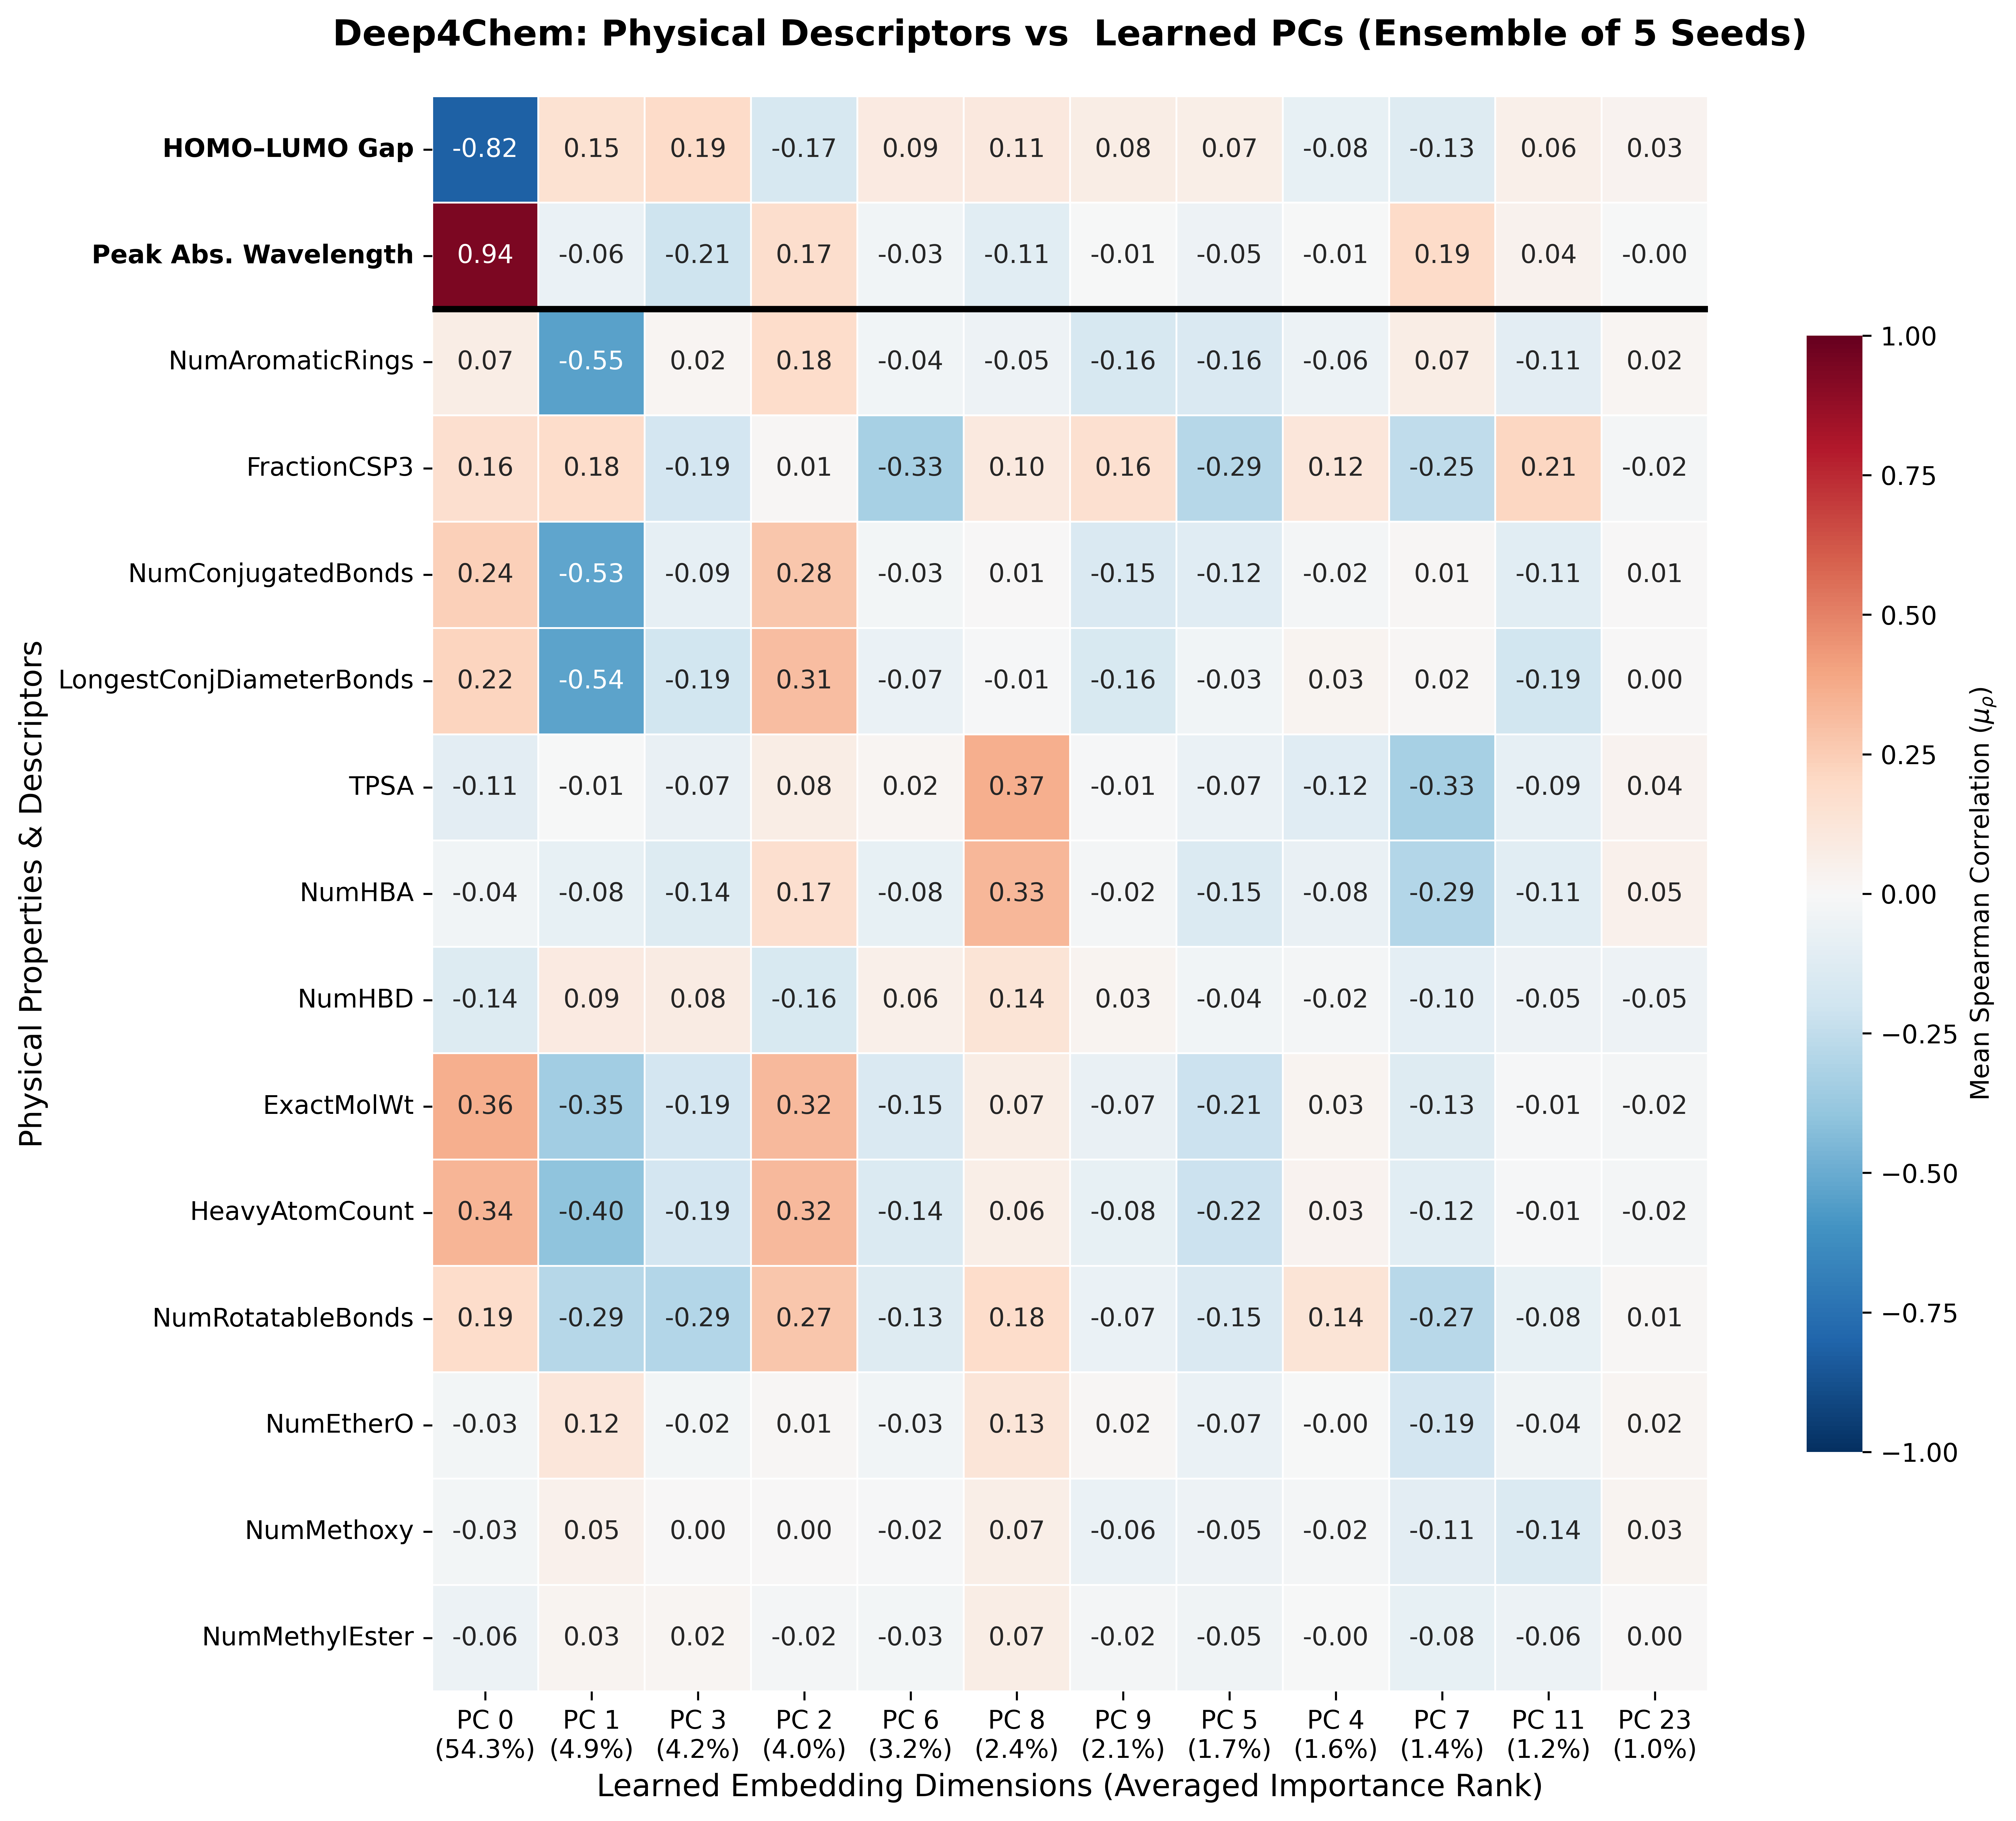
\includegraphics[width=0.8\textwidth]{figures/deep4chem-pc-physchem-heatmap.png}
\caption{\textbf{Consensus Interpretability Map: Learned PCs vs Physics.} 
Aligned Spearman rank correlations between the top 12 predictive principal components (PCs) and physicochemical descriptors across an ensemble of 5 seeds. PCs are ordered by averaged XGB feature importance. The horizontal divider separates structural descriptors from the photophysical targets, HOMO--LUMO gap and peak absorption wavelength.}
\label{fig:pc-physchem-heatmap}
\end{figure*}

\subsection{Chemical Interpretation of Principal Components}
\paragraph{$PC_0$: The Effective Conjugation Axis.}
As visualized in Figure~\ref{fig:abs-vs-pc0}, $PC_0$ can be interpreted as a learned coordinate for \textbf{``effective conjugation length''}. It separates molecules not just by the number of double bonds, but by their ability to delocalize electrons. Low $PC_0$ values correspond to torsionally twisted or interrupted $\pi$-systems, while high $PC_0$ values correspond to extended, planar architectures that promote efficient orbital overlap. The saturation of $\lambda_{\max}$ at high $PC_0$ values mirrors the physical ``saturation of redshift'' observed in long conjugated polymers~\cite{meier1997effective}, suggesting that the model has learned latent axes exhibiting behaviour consistent with known non-linear physics of delocalization without explicit supervision.

\begin{figure*}[t]
  \centering
  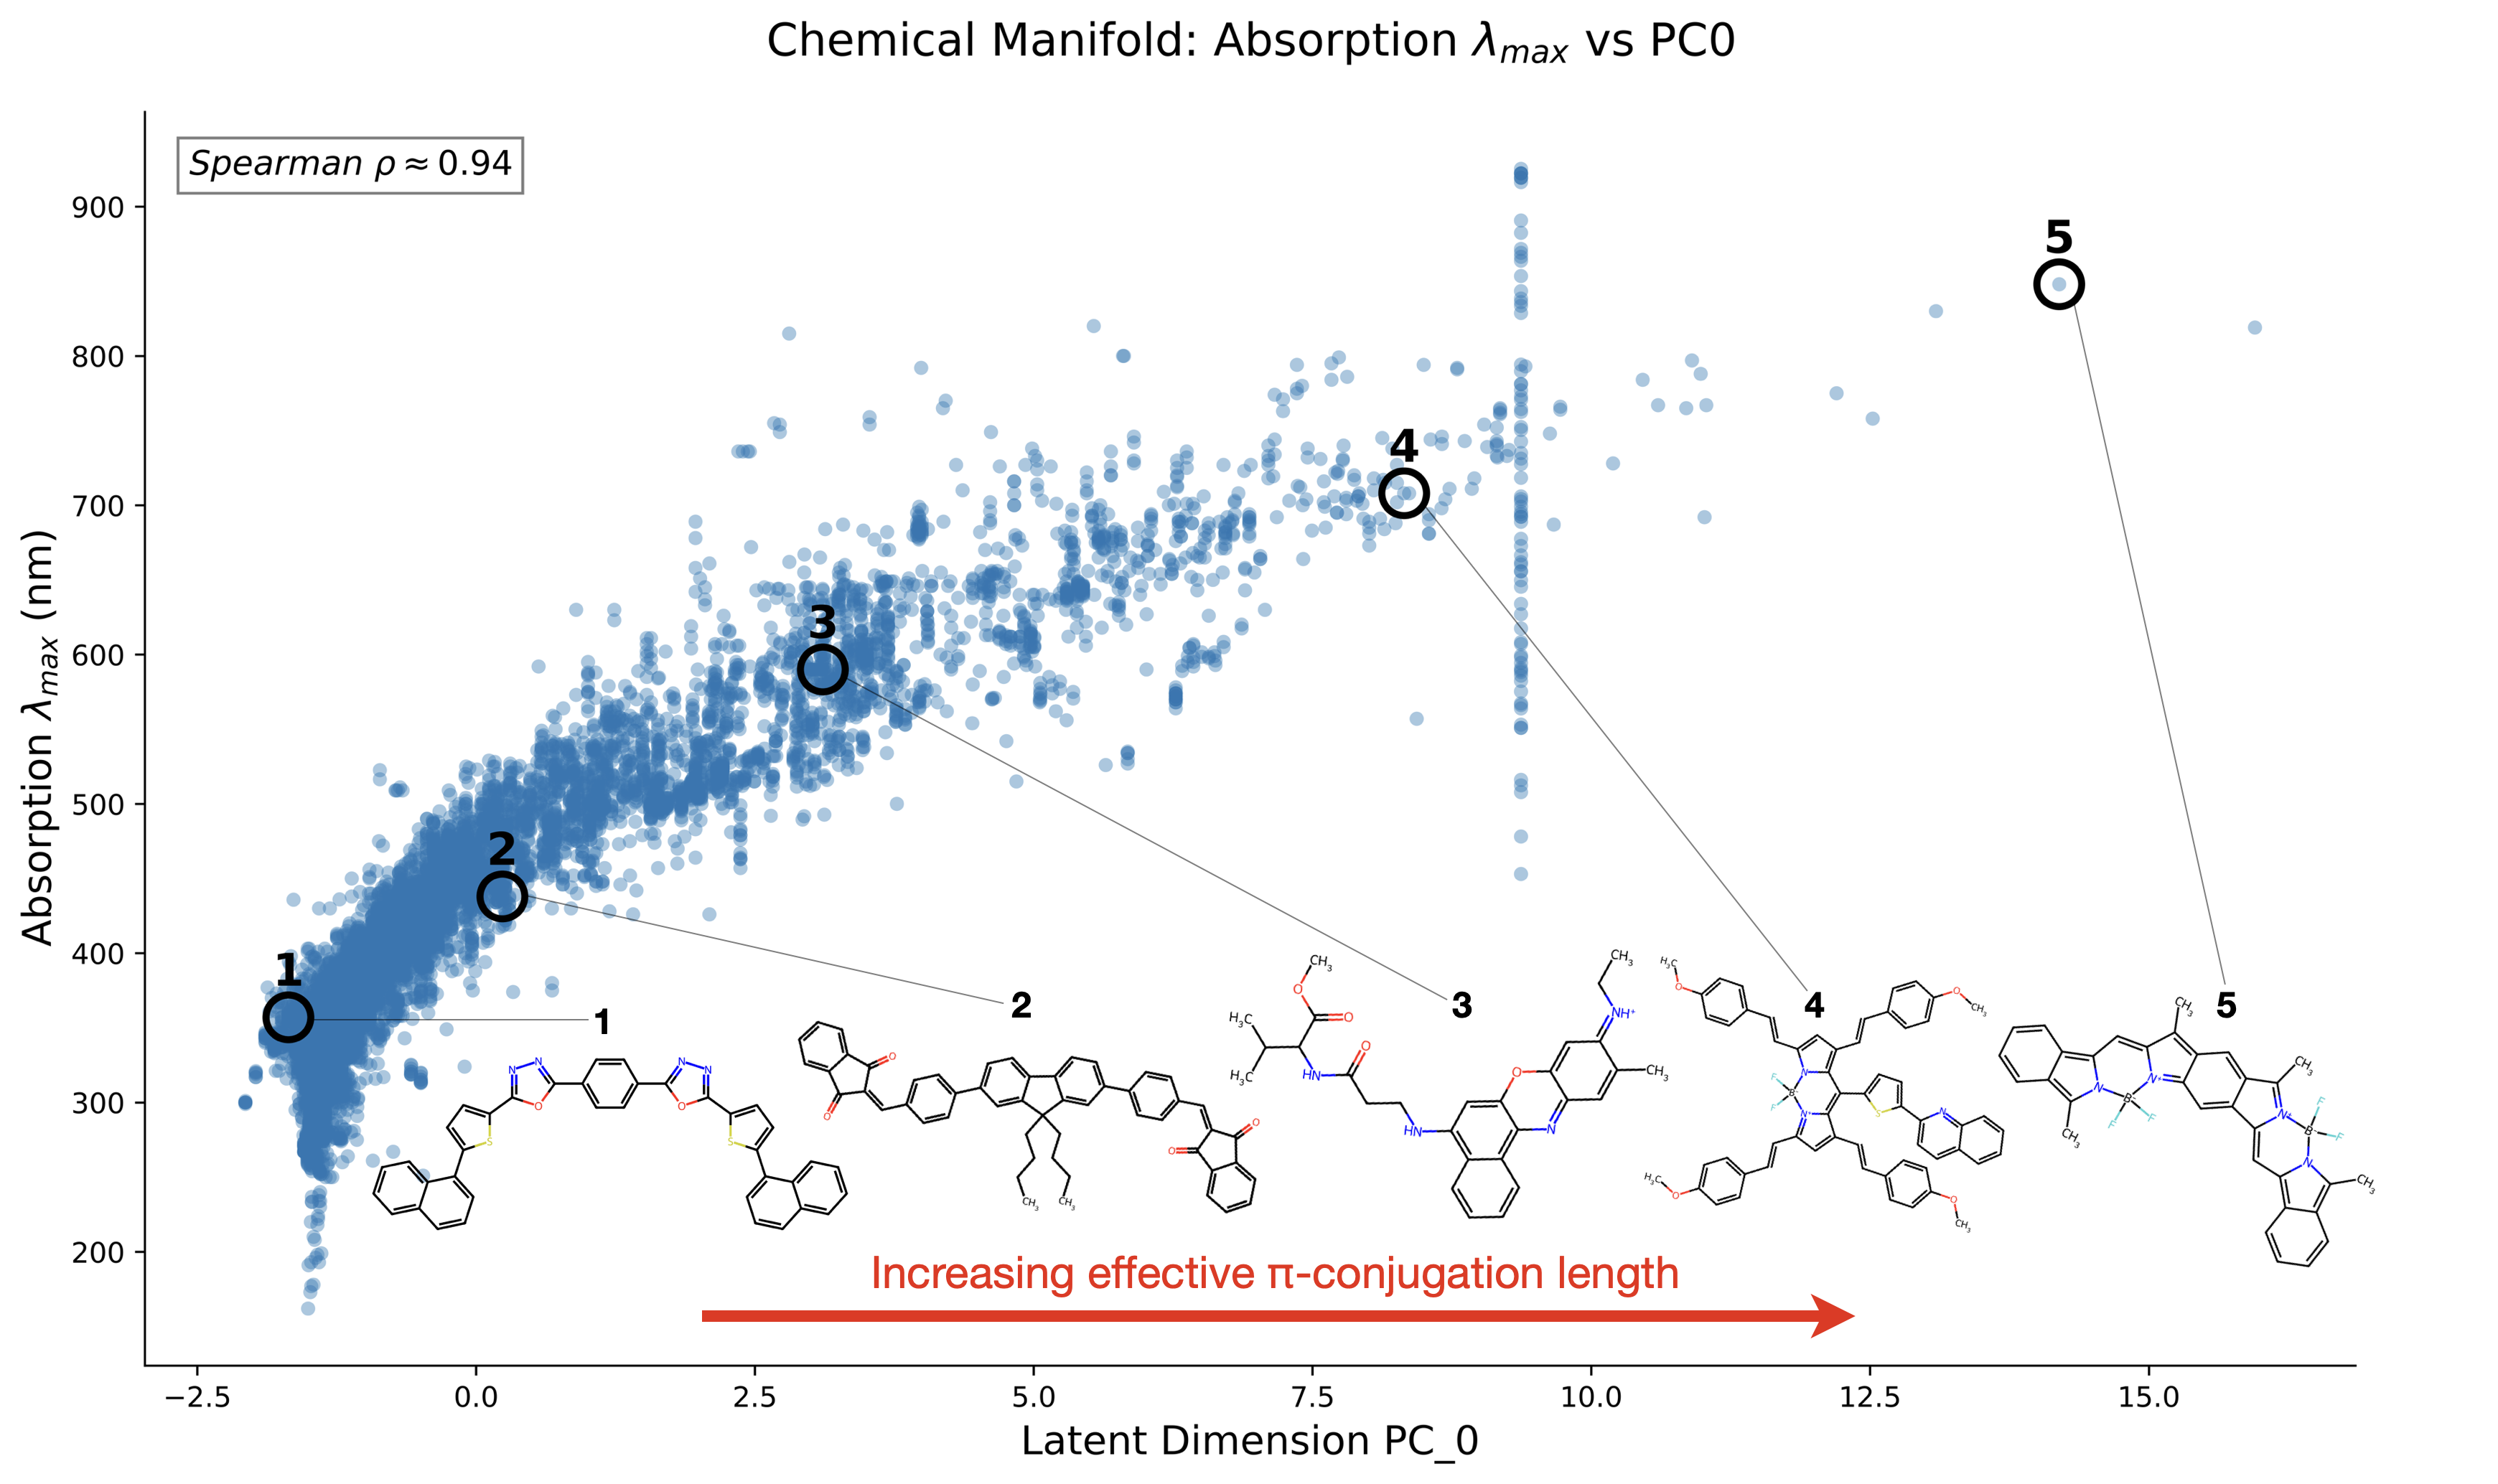
\includegraphics[width=0.9\textwidth]{figures/abs-vs-pc0.png}
  \caption{\textbf{Chemical manifold visualization showing the relationship between absorption $\lambda_{\max}$ and the dominant latent dimension $PC_0$.} The axis corresponds to ``effective conjugation length'': low values indicate interrupted or localized $\pi$-systems, while high values indicate extended, planar delocalization.}
  \label{fig:abs-vs-pc0}
\end{figure*}


\paragraph{Secondary Structural and Environmental Axes.}
Beyond the dominant electronic axis, several secondary components encode orthogonal structural and environmental factors. $PC_1$ primarily reflects aromaticity and conjugated topology, exhibiting negative correlations with \textit{NumAromaticRings} ($\rho = -0.55$) and \textit{LongestConjChain} ($\rho = -0.54$), while $PC_2$ tracks overall molecular size and flexibility, correlating with \textit{ExactMolWt} ($\rho = 0.32$), \textit{HeavyAtomCount} ($\rho = 0.32$), and \textit{NumRotatableBonds} ($\rho = 0.27$). 

Additionally, $PC_8$ appears to reflect polarity and solvation effects, correlating with topological polar surface area and hydrogen-bonding capacity. These dimensions adjust the predicted absorption wavelength around the dominant shift captured by $PC_0$, suggesting that the model distinguishes electronic delocalization from substituent-driven polarity and solvation effects (see Supporting Information, Figures~\ref{fig:si_hexbins} and~\ref{fig:pc8-vs-pc0}).

While several principal components have clear and chemically meaningful interpretations, not all latent directions exhibit strong correlations with the descriptors examined here. This is expected: PCA is a linear projection of a highly nonlinear learned representation, and individual components may encode interactions or higher-order structure not captured by standard physicochemical descriptors. The fact that multiple dominant components align so strongly with fundamental electronic and structural quantities is therefore notable. Additional analyses and tentative interpretations of lower-correlation components are provided in the Supporting Information.


\paragraph{Orthogonality of Electronic and Structural Factors.}
To examine the separation of electronic and structural effects, we perform a counterfactual analysis (Figure~\ref{fig:counterfactuals}). By projecting pairs of molecules (in a fixed solvent) that differ by single structural edits onto the aligned global $PC_0$ axis, we observe two distinct trajectories:

\begin{itemize}
    \item \textbf{Conjugation Extension and Aromatic Fusion (e.g., Bibenzyl $\to$ Stilbene; ``Broken Pentacene'' $\to$ Pentacene):} Structural edits that physically extend the conjugated network (linking double bonds or fusing aromatic rings) result in large displacements along the $PC_0$ axis, driving the expected redshift~\cite{yamaguchi2008pi, adachi1998relationship}.
    \item \textbf{Electronic Push-Pull (e.g., \textit{para}-Nitro-substitution):} Edits that induce charge transfer without extending the $\pi$-chain (e.g., donor-acceptor substitutions) produce vertical shifts in predicted $\lambda_{\max}$ (red or blue depending on the solvent), with minimal displacement along $PC_0$~\cite{yokoyama1984effects, maximo2024absorption, szatylowicz2017classical}.
\end{itemize}

These trends suggest that the latent representation separates wavelength shifts associated with the extent of $\pi$-conjugation (captured by $PC_0$) from those associated with substituent-induced charge transfer (captured by secondary dimensions), without requiring explicit physical supervision.

\begin{figure*}[t]
  \centering
  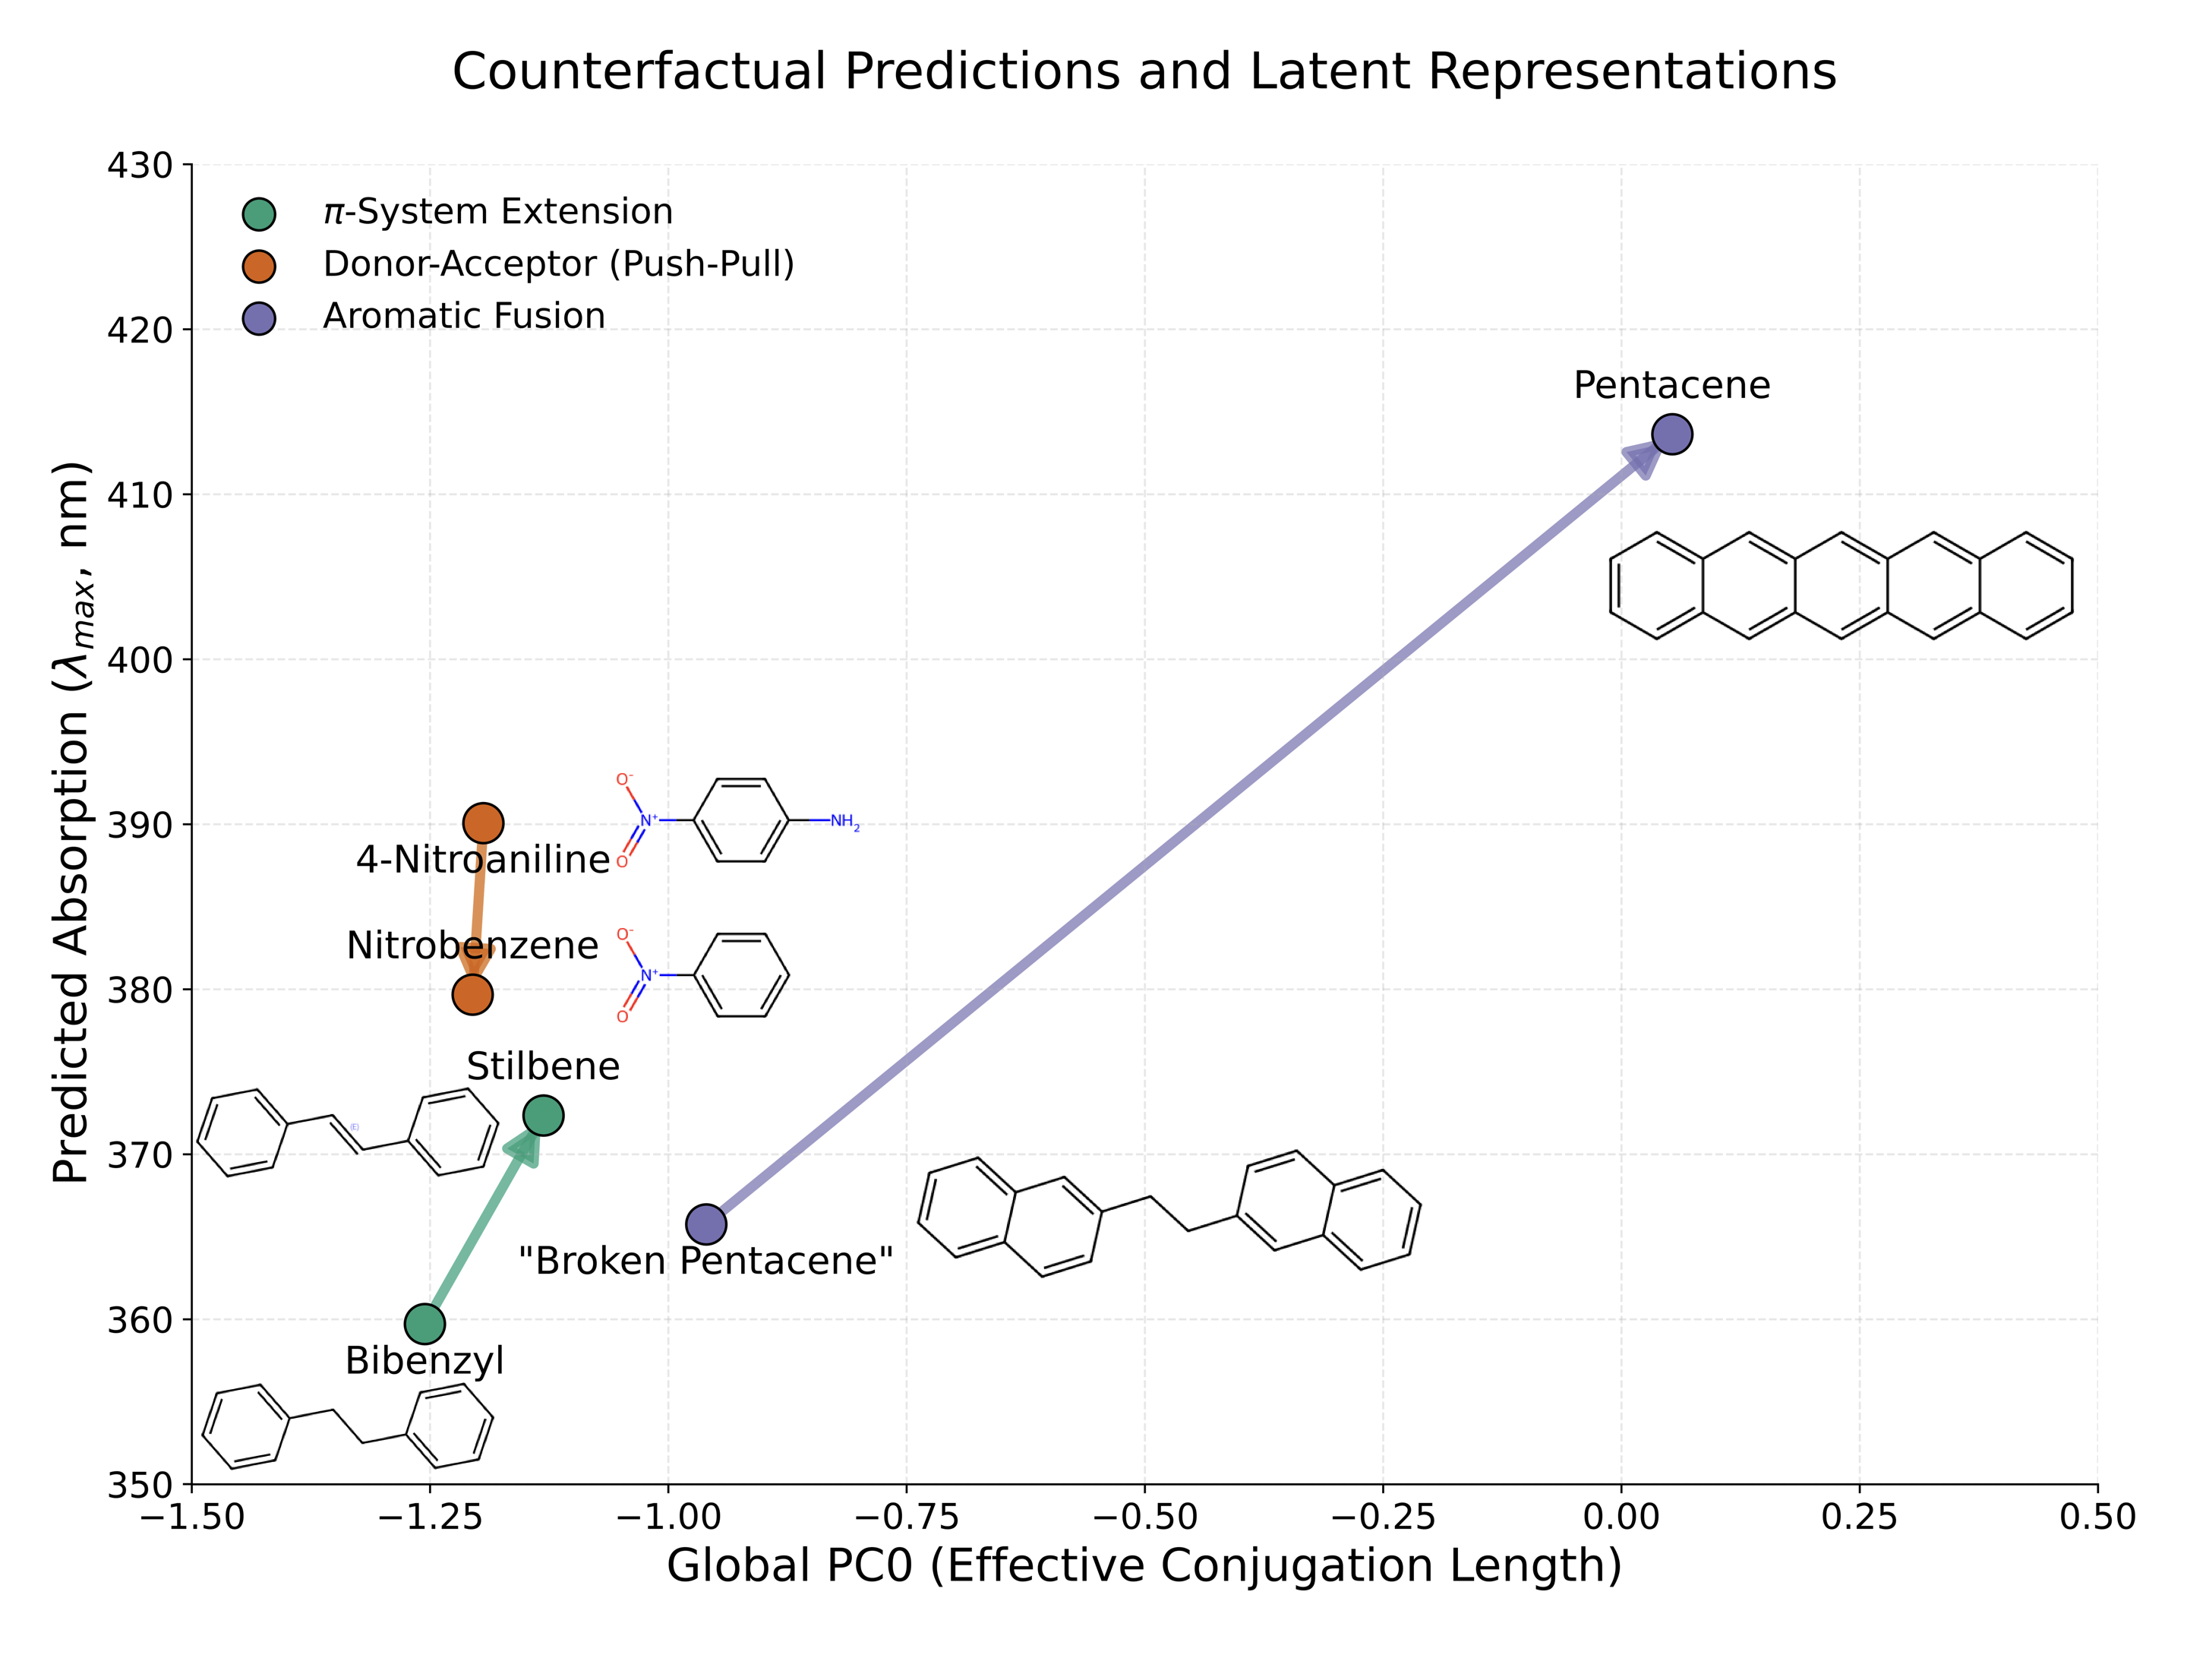
\includegraphics[width=0.9\textwidth]{figures/latent_space_interpretation_counterfactuals.png}
  \caption{\textbf{Counterfactual interpretation of the learned latent space.} 
  Latent embeddings for chemically matched pairs are projected onto the global $PC_0$ axis. Each arrow denotes a structural modification while keeping solvent constant. The horizontal axis ($PC_0$) tracks the effective conjugation length, while the vertical axis shows predicted $\lambda_{\max}$.}
  \label{fig:counterfactuals}
\end{figure*}

\section{Conclusion}
Data scarcity remains the primary bottleneck for applying deep learning to experimental photophysics. In this work, we showed that hybrid architectures can improve performance in this setting. By replacing the standard neural head of a trained D-MPNN with a post-hoc XGBoost model, we achieved relatively consistent improvements in absorption wavelength prediction across low-to-mid data regimes ($N \lesssim 1000$), particularly under rigorous scaffold splits that simulate realistic discovery scenarios.

\paragraph{Mechanisms of Stability and Interpretability.}
Our analysis identifies two distinct mechanisms driving this advantage. First, variance decomposition revealed that in small-data regimes, the mapping from learned representations to molecular properties is underdetermined; the hybrid model appears to stabilize this mapping by imposing the structural regularization of decision trees, effectively pruning the high-variance error component associated with neural heads. Second, we showed that the D-MPNN encoder, even when trained on limited data, learns a latent space that aligns with physically meaningful structure. The dominant principal component ($PC_0$) spontaneously aligns with the concept of ``effective conjugation length,'' separating extended $\pi$-conjugation from substituent-driven electronic effects. This suggests that the model’s predictive performance is driven in part by representations aligned with known physical factors, rather than relying solely on dataset-specific correlations.

\paragraph{Practical Implications.}
These findings suggest a practical workflow for molecular screening in low-data settings. Since fitting an XGBoost head on fixed embeddings incurs virtually negligible computational cost, practitioners can leverage the hybrid approach to maximize predictive stability in data-scarce regimes without sacrificing the scalability of end-to-end learning as datasets grow. Furthermore, our transfer learning results indicate that this strategy is particularly effective when adapting pretrained models to chemically similar downstream tasks (e.g., Deep4Chem $\to$ ChemFluor), though its utility diminishes under severe domain shift (e.g., Deep4Chem $\to$ DSSCDB).

\paragraph{Limitations and Future Directions.}
Several open challenges point toward future research.
\begin{itemize}
    \item \textbf{Excited-State Physics:} The hybrid advantage was less systematic for emission prediction. This likely reflects the fact that ground-state graphs do not explicitly encode excited-state relaxation or solvent reorganization energies. Future work should explore integrating low-cost conformational sampling or solvent-aware message passing to better constrain these dynamic effects.
    \item \textbf{Domain Adaptation:} While transfer learning succeeded for structurally overlapping datasets, it failed under significant distribution shift. Addressing this will likely require more principled domain adaptation techniques under data scarcity, such as adversarial pretraining or uncertainty-weighted fine-tuning, rather than simple parameter transfer.
    \item \textbf{Feature Integration:} An additional direction is to evaluate the integration of learned embeddings with physicochemical descriptors within the hybrid framework. Tree-based models naturally accommodate heterogeneous feature sets, suggesting that hybrid approaches may provide a practical mechanism for incorporating complementary domain knowledge in low-data regimes. A controlled comparison with end-to-end models trained on the same augmented inputs is required to determine whether this flexibility translates into improved predictive performance.
    \item \textbf{Scope of Properties:} Extending this analysis to intensive properties like quantum yield or fluorescence lifetime, which depend heavily on non-radiative decay pathways, will further clarify the boundaries of graph-based representation learning.
\end{itemize}

Ultimately, this work supports the use of the hybrid D-MPNN$\rightarrow$XGBoost framework as a strong and practical baseline for optical property prediction in low-data regimes. By combining the representational power of graph neural networks with the robust inference of classical machine learning, it provides a scalable and computationally efficient approach that remains grounded in chemically meaningful structure.
